\documentclass[a4paper,11pt]{article}
\usepackage{fullpage}
\usepackage[english]{babel}
\usepackage{amsmath,amsfonts,amssymb,graphicx,amsthm}

\usepackage{cite}
\usepackage{xcolor}

\newtheorem{theorem}{Theorem}[section]
\newtheorem{lemma}[theorem]{Lemma}
\newtheorem{corollary}[theorem]{Corollary}
\newtheorem{definition}[theorem]{Definition}


\graphicspath{{./fig/}}
\newcommand{\eps}{\varepsilon}
\newcommand{\N}{\mathbb{N}}
\newcommand{\R}{\mathbb{R}}
\newcommand{\etal}{\emph{et al.}\xspace}
\newcommand{\?}{\mskip1.5mu}
\newcommand{\Patrascu}{P\v{a}tra\c{s}cu\xspace}
\def\..{\,\mathpunct{\ldotp\ldotp}} % Middle stuff for intervals. Usage: \..
\DeclareMathOperator{\lcp}{lcp} % longest common prefix
\DeclareMathOperator{\lca}{lca} % least common ancestor
\DeclareMathOperator{\exit}{exit}
\DeclareMathOperator{\lrange}{\ell}
\DeclareMathOperator{\rrange}{r}
\DeclareMathOperator{\extent}{extent}
\DeclareMathOperator{\Pref}{Pref}
\DeclareMathOperator{\pred}{pred}
\DeclareMathOperator{\fbs}{FBS}




\usepackage[ruled,noend,linesnumbered,algosection]{algorithm2e}
\newenvironment{alg}{
  \begin{algorithm}[htbp]
    \DontPrintSemicolon
    \SetKwInput{KwIn}{input}
    \SetKwInput{KwOut}{output}
  }{\end{algorithm}}

\newcommand{\aremark}[3]{\textcolor{blue}{\textsc{#1 #2:}}
  \textcolor{red}{\textsf{#3}}}
\newcommand{\djamal}[2][says]{\aremark{Djamal}{#1}{#2}}
\newcommand{\paolo}[2][says]{\aremark{Paolo}{#1}{#2}}
\newcommand{\marcel}[2][says]{\aremark{Marcel}{#1}{#2}}
\newcommand{\wolfgang}[2][says]{\aremark{Wolfgang}{#1}{#2}}


  

\title{TBD\footnote{
Preliminary versions appeared as 
D. Belazzougui, P. Boldi, and S. Vigna. 
\emph{Predecessor search with distance-sensitive query
time}. \texttt{arXiv:1209.5441}, 2012
and 
M. Ehrhardt and W. Mulzer.  \emph{Delta-Fast Tries: Local 
Searches in Bounded Universes with Linear Space}. Proc.~15th WADS,
2017.  WM was partially 
supported by DFG project MU/3501-1 and ERC StG 757609.}}

\author{Djamal Belazzougui\thanks{Universit\'e Paris 
        Diderot---Paris 7, France,
        \texttt{djamal.belazzougui@gmail.com}}
        \and
        Paolo Boldi\thanks{Universit\`a degli Studi di Milano, Italy, 
	\texttt{boldi@dsi.unimi.it}}
        \and
        Marcel Ehrhardt\thanks{Institut f\"ur Informatik, Freie 
	Universit\"at Berlin,
        \texttt{\{marehr, mulzer\}@inf.fu-berlin.de}}
        \and 
        Wolfgang Mulzer\footnotemark[4]
        \and 
        Sebastiano Vigna\thanks{Universit\`a 
	degli Studi di Milano, Italy, 
	\texttt{vigna@acm.org}}
        }
\date{}
%---------------------------------------------------------------------

\begin{document}
\maketitle

\begin{abstract}
\wolfgang{TODO}
\end{abstract}

\iffalse
\section{Sensitive Abstract}
A \emph{predecessor (successor) search} finds the largest 
element $x^-$ smaller than the input string $x$ (the smallest 
element $x^+$ larger than or equal to $x$, respectively) out of 
a given set $S$; in this paper, we consider the static case 
(i.e., $S$ is fixed and does not change over time) and assume 
that the $n$ elements of $S$ are available for inspection. We 
present a number of algorithms that, with a small additional 
index (usually of $O(n\log w)$ bits, where $w$ is the string 
length), can answer predecessor/successor queries quickly and 
with time bounds that depend on different kinds of \emph{distance},
improving significantly several results that appeared in the 
recent literature. Intuitively, our first result has a running 
time that depends on the distance between $x$ and $x^\pm$: 
it is especially efficient when the input $x$ is either very 
close to or very far from $x^-$ or $x^+$; our second result 
depends on some global notion of distance in the set $S$,
and is fast when the elements of $S$ are more or less equally 
spaced in the universe; finally, for our third result we rely 
on a \emph{finger} (i.e., an element of $S$) to improve upon 
the first one; its running time depends on the distance between 
the input and the finger.
\fi

\section{Introduction}

Predecessor searching is one of the oldest problems 
in theoretical computer science~\cite{CormenLeRiSt09,Knuth98}: 
let $U$ be a totally ordered universe. The task is 
to store a subset $S$ of $U$, while supporting 
\emph{predecessor} and \emph{successor} queries: 
given $q \in U$, find the largest element in $S$ 
smaller than $q$ (the predecessor of $q$) or the 
smallest element in $S$ larger than $q$ (the 
successor of $q$). In the \emph{dynamic} version, 
we also allow modification of $S$ by insertion 
and/or deletion of elements from $U$.

For the predecessor searching problem, the model 
of computation is of particular importance. In 
the \emph{word-RAM} model, all input elements 
are represented by $w$-bit \emph{words}, where 
$w \in \N$ is a parameter. Thus, we can assume 
that the universe is $U = \{0, \dots, 2^{w}-1\}$. 
Moreover, we assume that $w$ 
is a power of $2$. This does not lead to any 
loss of generality, since our asymptotic bounds 
are not affected by changing $w$ by a factor of 
at most $2$. The word-RAM model allows us to 
manipulate the data words at the bit level, 
in constant time per operation. A classic 
method for predecessor searching on the 
word-RAM is due to van Emde Boas, who described 
a dynamic data structure that requires $O(n)$ words
of space and supports insertions, deletions, and 
predecessor queries in 
$O(\log w) = O(\log\log |U|)$ 
time~\cite{vEmdeBoas77,vEmdeBoasKaZi76,CormenLeRiSt09}.
Here, $n$ denotes the current size of the
(dynamically changing) set $S$. This data 
structure is now commonly known as the 
\emph{van-Emde-Boas tree}~\cite{CormenLeRiSt09}.

For the \emph{pointer machine} model of computation, 
which is more restrictive than the word-RAM, it has 
been known for a long time that a variant of the 
van-Emde-Boas tree provides optimal 
performance~\cite{MehlhornNaAl88,Mulzer09}.
For the word RAM, \Patrascu and Thorup~\cite{PatrascuTh06,PatrascuTh07} 
recently showed that structures similar to the 
van-Emde-Boas tree (e.g., $y$-fast tries~\cite{Willard83}) 
with query time $O(\log w)$ are optimal, assuming that 
we desire the space requirement to be linear in the 
size of $S$. More generally, the lower bound of 
\Patrascu and Thorup~\cite{PatrascuTh06,PatrascuTh07} 
encompasses several regimes, depending on the 
space that is available for the data structure.
For instance, another case is realized by exponential 
trees~\cite{AnderssonTh07}.\wolfgang{Which case is this?} 
For a comprehensive discussion of the literature, we refer
the reader to Mihai \Patrascu's thesis~\cite{Patrascu08}.

Thus, the worst-case complexity of the predecessor 
searching problem has been settled. However, there is 
still room for improvement: first, suppose we are 
given the original set $S$ as a sorted array. Then,
we may desire a data structure that requires 
only \emph{sublinear} additional space and answers
predecessor queries for $S$ in optimal time; second, 
we may ask for a more nuanced guarantee on the query 
time that could depend on the structure of $S$ or on 
the relationship between the query element $q$ and 
the set $S$. More concretely, suppose our data 
structure currently contains the set $S \subseteq U$. 
To model the structure of $S$, we write $\Delta_M$ 
and $\Delta_m$ for the maximum and minimum distance 
between any two consecutive elements of $S$.
Furthermore, let $q \in U$ be the query element,  
and write
\[
  q^+ := \min\{s \in S \mid s \geq q \}
\]
and
\[
q^- := \max\{s \in S \mid s < q \}
\] 
for the 
successor and the predecessor of $q$ in $S$.
Then, we have several ways to model the
relationship between $S$ and $q$: 
let 
\[
d(q, S) = \min\big\{|q - q^-|, |q - q^+|\big\}
\]
and 
\[
D(q, S) = \max\big\{|q - q^-|, |q - q^+|\big\}.
\]
We call $d(q,S)$ the \emph{short distance} and 
$D(q, S)$ the \emph{long distance} between $q$ and 
$S$.
The short distance $d(q, S)$ is small when $q$ is 
close to an element of $S$, whereas $w - \log D(q, S)$
is small when $q$ is far from either $q^+$
or $q^-$. 

In 2013, Bose~\etal~\cite{BoseDoDuHoMo13} described
a word-RAM data structure for the dynamic predecessor
problem that is \emph{local} with respect to updates
and queries.
In particular, their structure can answer predecessor 
and successor queries and perform updates 
in $O\big(\log\log d(q, S)\big)$ time.
It requires $O\big(n w \log\log w)$ bits 
of space, where $n = |S|$ is the size of the 
current set. Bose~\etal apply their structure 
to obtain a fast data structure for approximate nearest 
neighbor queries in low dimensions and for answering
dominance and range searching queries on a grid~\cite{BoseDoDuHoMo13}.

Here, we describe data structures for the
static and dynamic predecessor problem
on the word RAM that provide significant 
improvements over previous bounds.\footnote{Our 
space bounds are always given as
number of bits \emph{in addition} to those needed for 
representing $S$.} 

\begin{enumerate}
  \item We match the static worst-case search time 
  $O\big(\log\log d(q, S)\big)$
  of Bose~\etal~\cite{BoseDoDuHoMo13}, but our index requires 
  just $O(n\log w)$ additional bits of space (and thus overall 
  linear space).
  \item Using $O(nw)$ bits, we can also match the dynamic
  update and search time $O\big(\log\log d(q, S)\big)$
  of Bose~\etal~\cite{BoseDoDuHoMo13}.
  \item We improve exponentially over the \emph{interval-biased search
  trees} of Bille~\etal~\cite{BilleLaRaSaSaWe15}, answering 
  predecessor queries in time\footnote{The
  bound of Bille~\etal~\cite{BilleLaRaSaSaWe15} is 
  $O(w - \log(q^+ - q^-))$. Our 
  proofs work even replacing $D(q, S)$ with $q^+ - q^-$, but 
  the difference is immaterial as $q^+ - q^-\leq 2D(q, S)$, and 
  we find the duality with the previous bound more intuitive.} 
  $O\big(\log(w - \log D(q, S))\big)$, with 
  $O(n\log w)$ additional bits.
  \item We improve exponentially over the \emph{interpolation
  search} of Demaine~\etal~\cite{DemaineJoPa04}, answering
  predecessor queries in time 
  $O\left(\log\log(\Delta_M / \Delta_m)\right)$, with
  $O(n\log w)$ additional bits.
  \item Finally, with slightly more (but still sublinear) space 
  we can exploit a \emph{finger} $r \in S$ to speed up our third 
  result to $O\left(\log(\log|q - r| - \log D(q, S))\right)$, which is in
  some cases better than the bound reported
  by Andersson and Thorup~\cite{AnderssonTh07}, and improves 
  exponentially over interval-biased search trees, which need 
  time  
  $O\left(\log(2^w - y) - \log D(q, S)\right)$~\cite{BilleLaRaSaSaWe15}.
\end{enumerate}
We remark that a combination of the first
and the third result shows that static predecessor 
search can be performed in time  
$O\left(\log \min \{\,\log d(x,S),w-\log D(x,S)\,\}\right)$ 
with $O(n \log w)$ additional bits. Our 
results are obtained starting from a refined version of
\emph{fat binary search in a $z$-fast trie}~\cite{BelazzouguiBoPaVi09} 
in which the initial search interval can be specified under 
suitable conditions, confirming the intuition that fat
binary search can be used as a very versatile building block 
for data structures.

\section{Notation and Tools}
\label{sec:notation}

\paragraph{Basic Notations.}
We use $\log x$ to denote the binary logarithm, and we set 
$\log x := 1$, for $x \leq 2$.
We write $\eps$ for the empty string. For $k \in \N$, we denote by 
$\{0, 1\}^k$ the set of all binary strings of length $k$, by 
$\{0,1\}^+ := \bigcup_{k = 1}^{\infty} \{0, 1\}^k$ the set of all
nonempty finite binary strings, and by 
$\{0,1\}^* := \{0, 1\}^+ \cup \{\eps\}$ the set of all finite binary 
strings. The length of $q \in \{0, 1\}^*$ is denoted by $|q|$.
For a string $q \in \{0, 1\}^*$ and $a, b \in \N$ with $a \leq b$, 
we write $q[a, b]$ for the substring of $q$ starting at position
$a$ and ending at position $b$.  The indices start from $0$. 
We abbreviate $q[a, a]$ as $q[a]$. For two binary strings 
$q, r \in \{0,1\}^*$, we write $q \preceq r$ to indicate that $q$ is 
a prefix of $r$, and $q \prec r$ to indicate that $q$ is a proper 
prefix of $r$. 
Given a set $S \subseteq \{0, 1\}^*$, we write 
$\Pref(S) = \{p \in \{0, 1\}^* \mid \exists s \in S: p \preceq s\}$
for the set of all prefixes of the strings in $S$.
Given a string 
$q \in \{0,1\}^+$, we denote with $q + 1$ and $q - 1$ the strings in 
$\{0, 1\}^{|q|}$ that come before and after $q$ in lexicographic 
order. We use the convention that $0^k - 1 = 1^k + 1 = \bot$, for 
$k \in \N$, since then the predecessor and the successor do 
not exist. 

\paragraph{The Word RAM.}
Let $w \in \N$ be a power of two. We work in the standard word RAM 
model with word-length $w$. 
\wolfgang{Add something about the mcb operation?}

\paragraph{Predecessor and Successor Queries.}
Given a set $S \subseteq \{0, 1\}^w$ of $n$ binary strings of 
length $w$, we consider $S$ to be ordered according to the 
lexicographic order, and for $q \in \{0, 1\}^w$, we set
\begin{align*}
     q^- &= \max \{r \in S \mid r < q\} && 
        \text{(the \emph{predecessor} of $q$ in $S$)} \\
     q^+ &= \min \{r \in S \mid r \geq q\?\} && 
       \text{(the \emph{successor} of $q$ in $S$)}.
\end{align*}
If the maximum or minimum does not exist, we set $q^- = \bot$ or 
$q^+ = \bot$.  A \emph{predecessor} or \emph{successor query} is
given by a string $q \in \{0, 1\}^w$, and the answer is $q^-$ or 
$q^+$. In fact, we shall focus exclusively on predecessor queries. 
This does not affect the generality of our results,
also because our algorithms actually return the \emph{rank} of the 
predecessor in $S$, and thus are in principle more informative 
than basic predecessor operations
(e.g., the successor can be immediately computed by incrementing 
the resulting index).

\paragraph{Hash Maps.}
Our data structure makes extensive use of
hashing. In particular, we will maintain several
succinct hash tables that store additional
information for supporting fast queries.
For this, we will use a hash table described
by Demaine~\etal~\cite{DemaineMePaPa06}.
The following theorem summarizes the properties
of their data structure.

\begin{theorem}\label{thm:succinct_retrieval_only_hashtable}
For any $r \geq 1$, there exists a dynamic dictionary that
stores entries with keys from $U$ and with associated
values of $r$ bits each.
The dictionary supports updates and queries in $O(1)$ time,
using $O(n \log\log (|U|/n) + nr)$ \emph{bits} of space.
The bounds for the space and the queries are
worst-case, the bounds for the updates hold with
high probability.\qed
\end{theorem}

\wolfgang{TO CHECK: Do we need the full-randomness assumption in 
Theorem 2.1? Check about multiplication?}

\wolfgang{Cite a specific theorem for this, similar to 
  Theorem~\ref{thm:succinct_retrieval_only_hashtable}?}
\wolfgang{Check whether we actually need the following? Is the
$O(n \log w)$ overhead from Theorem 2.1 enough?}
We assume to be able to store a constant-time $r$-bit function on 
$n$ keys using $rn+cn +o(n)$ bits, for some constant $c\geq 0$: the 
function may return arbitrary values outside of its domain (for 
practical implementations see~\cite{BelazzouguiBoPaVi11}).

\section{Z-fast Tries} 

\subsection{Compressed Tries}
Our data structure is based on \emph{compressed
tries}~\cite{CormenLeRiSt09,Knuth98}. These are defined as
follows: let $S \subseteq \{0, 1\}^w$. The \emph{trie} $T'$ for $S$ 
is a binary tree of height $w$. Each node $v \in T'$ corresponds
to a bit string $e_v \in \{0,1\}^*$, called the \emph{extent} of $v$. 
The root has extent $\eps$. For each inner node $v$, the left child 
$u$ of $v$  has $e_u = e_v0$, and the right child $w$ of $v$ has 
$e_w = e_v1$ (one of the two children may not exist). The extents of
the leaves correspond to the elements of $S$, and the extents of the 
inner nodes are prefixes for the elements in $S$, see 
Figure~\ref{fig:trie}.

\begin{figure}
  \centering
  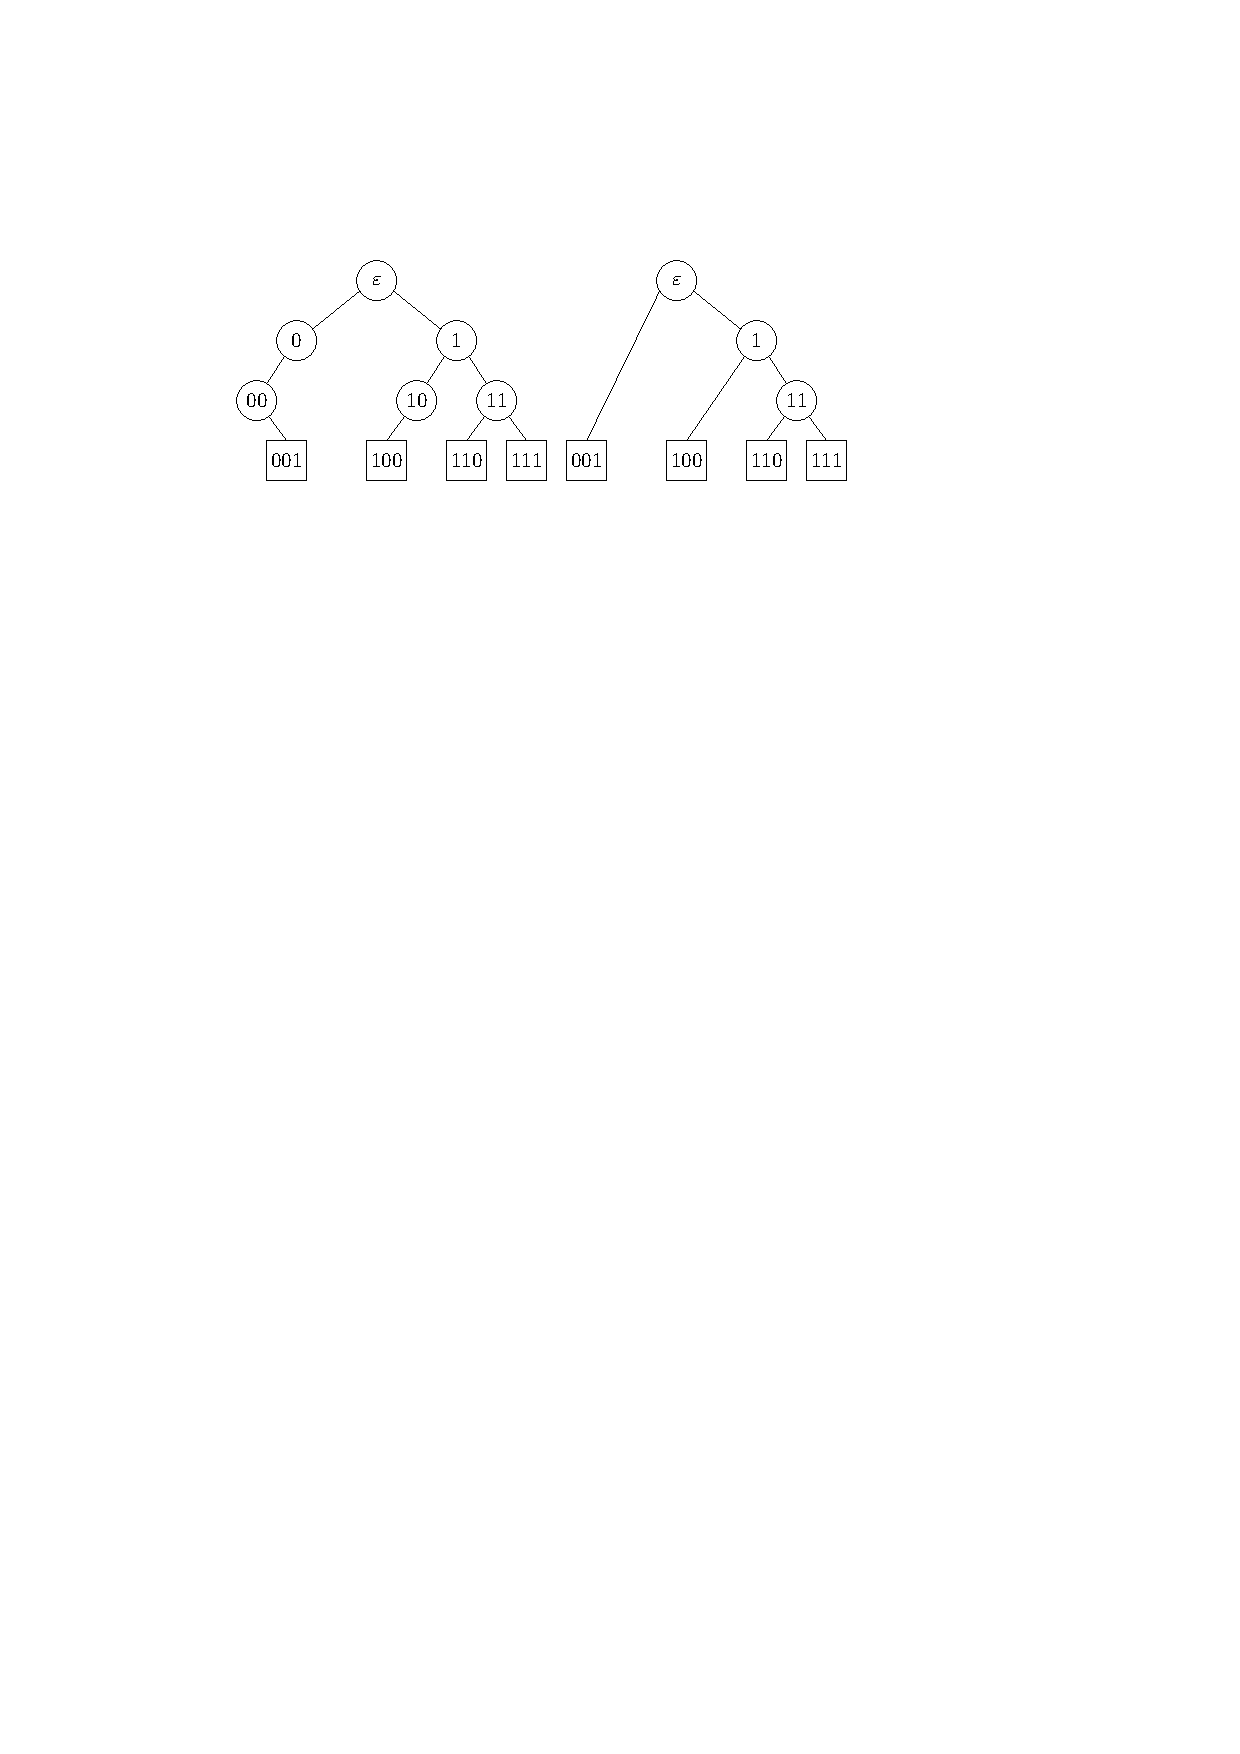
\includegraphics{trie}
  \caption{A trie (left) and a compressed trie (right) for the set 
  000, 100, 110, 111. The longest common prefix of 101 is  10. The 
  lca of 101 in the compressed trie
    is the node labeled 1.}
  \label{fig:trie}
\end{figure}

The \emph{compressed trie} $T$ for $S$ is obtained
from $T'$ by contracting each maximal path of nodes
with only one child into a single edge. 
The root of $T$ is corresponds to the highest node of $T'$ that has 
two children.  Each inner node in $T$ has exactly two children. 
Consequently, $T$ has $O(n)$ nodes. 
The extents of the nodes in $T$ are given by the longest 
extents along the corresponding compressed paths.
%Maybe somewhat unusually, in the following, the 
%\emph{height} and \emph{depth} of a node $v$ in $T$ 
%will refer to the corresponding
%height and depth in the (uncompressed) trie $T'$.
%This convention will make the description of the operations more
%convenient.

Let $v$ be a nonroot-node in the compressed trie $T$,
and suppose that $u$ is the parent of $v$ in $T$. Then, 
the extent $e_v$ of $v$ has the form $e_v = e_ubc_v$, 
where $e_u \in \{0, 1\}^*$ is the extent of $u$, $b \in \{0,1\}$ is 
a bit that indicates whether $v$ is the left or the right child
of $u$, and $c_v \in \{0, 1\}^*$ is called the \emph{compressed
path} of $v$. Both $e_u$ and $c_v$ may be empty, but $e_u$
can be empty only if $u$ is the root of $T$. 
We call $n_v = e_ub$ the \emph{name} of $u$.
For the root $v$, the extent $e_v$ may be empty, and we set
the compressed path $c_v = e_v$. Also, we set $n_v = \eps$.
We call an extent $e_v$ \emph{internal}, if $v$ is an internal
node of $T$.
For any node $v$ in $T$, the \emph{skip interval} of $v$ is 
$[1, |e_v|]$, if $v$ is the root, and $[|n_v|, |e_v|]$, otherwise.
Given a string $q \in \{0, 1\}^*$, with $|q| \leq w$, the 
\emph{exit node} of $q$, $\exit(q)$, is the unique node
$v$ in $T$ such that $n_v$ is a prefix of $q$ and either
$e_v = q$ or $e_v$ is not a prefix of $q$.
Figure~\ref{fig:ztrie} illustrates these definitions.

\begin{figure}[t]
\centering
\includegraphics[scale=.80]{zpred-1.mps}\qquad\raisebox{2cm}{\small
$T$~\begin{tabular}{c}
\fbox{\begin{tabular}{lcl}
0010 & $\to$ & $001001$\\
00100110 & $\to$ & $00100110100100$\\
\end{tabular}}\qquad
\end{tabular}
}
\caption{(above) A compressed trie, the 
related names, and the function $T$ of the associated 
z-fast trie. The skip interval for $\alpha$ is $[7\..13]$. 
Dashed lines show the end of the handles of internal nodes.}
\label{fig:ztrie}
\end{figure}

\subsection{Z-fast Tries and Fat Binary Search}
We recall some key definitions from~\cite{BelazzouguiBoPaVi09}:

\begin{definition}[2-fattest numbers and handles] 
\label{def:twofattest}
Let $a, b \in \N$, $a \leq b$. The \emph{2-fattest number} 
of the interval $[a, b]$ is the unique integer in $[a, b]$ 
that is divisible by the largest power of two. Equivalently, 
it is the integer with the largest number of trailing zeroes 
in its binary representation. The \emph{handle} $h_v$ of a 
node $v$ in a compressed trie is the prefix of $e_v$ whose 
length is the 2-fattest number of the skip interval of $v$
(see Figure~\ref{fig:ztrie}). If the skip interval of $v$ 
is empty (which can happen only at the root), we set 
$h_v = \eps$.
\end{definition}

We remark that if $c$ is the 2-fattest number of $[a, b]$, it 
is also the 2-fattest number in every subinterval of $[a, b]$ 
that contains it.

\begin{definition}[z-fast trie]
Let $S \subseteq \{0, 1\}^w$ be given, and let $T$ be the 
compressed trie for $S$. The \emph{z-fast trie on $S$} is 
the function $Z : \{0, 1\}^* \rightarrow \{0, 1\}^*$ which 
has $Z(h_v) = e_v$, for each internal node $v$ of $T$, and 
which maps any other string to an arbitrary internal extent
of $T$.
\end{definition}

Given the z-fast trie $Z$, we can determine very quickly
the name of the exit node for any query string $q \in \{0,1\}^+$.
For this, we use a variant of binary search, called 
\emph{fat binary search} see Algorithm~\ref{algo:query}. 
The algorithm locates the longest internal extent $e$ that is a 
proper prefix of $q$. For $e$, the name of $\exit(q)$ is obtained as
$q[0, |e| + 1]$. Given an initial search interval $[a,b]$, the 
fat binary search repeatedly splits it on its 2-fattest number, 
rather than on its midpoint. This makes the search order more
predictable among different starting intervals and thus allows 
for effective preprocessing.
The algorithm reported here, an extension of the 
result from~\cite{BelazzouguiBoVi10}, has two main features:
it imposes very weak requirements on $Z$, and it allows us to start 
the search on a small interval. The latter feature will be the key 
in obtaining our main results.

\begin{algorithm}
\KwIn{a string $q \in \{0,1\}^+$, an integer $a \in [0, |q|]$
such that $a = 0$ or $q[0, a - 1]$ is an internal extent of $T$, and
an integer $b \in [a, |q|]$ larger than the length of the longest 
internal extent of $T$ that is a proper prefix of $q$}
\KwOut{the name of $\exit(q)$}
\While{$b - a > 1$}{%
$c \gets $ the 2-fattest number in $[a + 1, b - 1]$\;
$e \gets Z(q[0, c - 1])$\;
\If{$c \leq |e| \wedge e \prec q$}{%
  \tcp{Move from $[a, b]$ to $[|e|,b]$}
 $a\gets |e|$\;
\label{alg1:reass1} 
} \Else{%
\tcp{Move from $[a, b]$ to $[a, c]$}
$b \gets c$\;
\label{alg1:reass2} 
}
}
\If{$a = 0 \wedge e_\text{root}\neq\eps$}{% 
  \Return $\eps$\;
} \Else{%
  \Return $q[0, a]$\;
}
\caption{Fat binary search in order to 
  determine the name of $\exit(q)$.}
\label{algo:query}
\end{algorithm}

\begin{lemma}\label{lem:correctness}
Let $e_0 = \eps$ and $e_1, e_2, \dots, e_t$ be the internal 
extents of $T$ that are \emph{proper} prefixes of $q$, ordered by 
increasing length.  Let $[a, b]$ be the interval maintained by 
Algorithm~\ref{algo:query}. Before and after each iteration, the 
following invariants are satisfied: 
\begin{enumerate}
    \item\label{enu:lema} $a = |e_j|$, for some $j$;
    \item\label{enu:lemb} $|e_t|< b$.
\end{enumerate}
Thus, at the end of the loop, $a = |e_t|$.
\end{lemma}

\begin{proof}
We begin with invariant (\ref{enu:lema}).
By assumption, the condition $a = |e_j|$, for some $j$, holds
initially. The condition is maintained whenever
$a$ is assigned a new value in line~\ref{alg1:reass1}. 
Indeed, suppose that currently $a = |e_j|$, for some $j$, and
that line~\ref{alg1:reass1} is reached. Then, since $e$ is an 
internal extent, since $|e_j| = a  < c  \leq |e|$, 
and since $e \prec q$, it follows that $e = e_k$, for some $k > j$.

Next, we consider invariant (\ref{enu:lemb}).
By assumption, the condition $|e_t| < b$ holds initially.
To show that the invariant is preserved,
suppose that at the beginning of an iteration of the
\textbf{while}-loop, we have $|e_t| < b$.
By invariant (\ref{enu:lema}), $a = |e_j|$, for some $j$.  
Let $v_{j+1}, \dots, v_{t}$ be the inner nodes in $T$ 
with $e_{v_k} = e_k$, for $k = j + 1, \dots, t$.
Then, the skip intervals of $v_{j+1}, \dots, v_t$ are 
pairwise disjoint, and their union is $[a + 1, |e_t|]$.
If $c \leq |e_t|$, then $c$ lies in the
skip interval of some $v_k$.
Since $c$ is 2-fattest in $[a + 1, b - 1]$, 
it is also 2-fattest in the skip interval of $v_k$. 
Hence, we have $q[0, c - 1] = h_{v_k}$ and 
$Z(q[0, c - 1]) = e_k$, 
which satisfies $c \leq |e_k|$ and $e_k  \prec q$. 
Thus, line~\ref{alg1:reass2} is executed only if $|e_t| < c$.
The invariant $|e_t| < b$ is preserved.
\end{proof}

\begin{theorem}
\label{thm:correctnessfbs}
Algorithm~\ref{algo:query} takes at most $\lceil\log(b-a)\rceil$
iterations
and finds the name of $\exit(q)$.
\end{theorem}

\begin{proof}
We first bound the number of iterations. Let 
$[\ell, r]$ be an interval that contains at most one multiple of 
$2^i$, and let $c$ be the 2-fattest number in $[\ell, r]$. Then, 
the two subintervals $[\ell, c - 1]$ and $[c + 1, r]$ each contain 
at most one multiple of $2^{i-1}$: if one interval contained two such 
multiples, it would also contain a multiple of $2^i$
in the interior, contradicting our assumption.
By induction, it follows that after splitting
at most $i$ times, the resulting interval has length at most one. 
Now, since an interval of length $k$ contains at most one multiple of 
$2^{\lceil\log k\rceil}$, the algorithm
has at most $\lceil\log(b-a)\rceil$ iterations.

Finally, if $t > 0$ then $q[0, |p_t|]$ is the name of $\exit(q)$.
Otherwise, $\exit(q)$ is the root (hence the special case in 
Algorithm~\ref{algo:query}).
\end{proof}

To find the 2-fattest number in an interval $[\ell + 1, r]$, for 
nonnegative integers $\ell < r$, we need 
an \texttt{msb}-operation.\footnote{More precisely, the 
2-fattest number in $[\ell, r]$ is 
$(1^w \texttt{ shl } 
\texttt{msb}(\ell \texttt{ xor } r)) \texttt{ and } r$. 
We write the interval boundaries as $[\ell +1 , r]$ instead of
$[\ell, r]$, since this allows for the most convenient formulation
of the operation.}
However, there is an alternative that does not need the most 
significant bit operation.  Starting from the interval $[\ell + 1, r]$
we set $i = \lceil\log(r - \ell)\rceil$ (trivially, we can find $i$ 
in time $O(\log(r -\ell))$).
Then we check, for decreasing $i$, whether 
$(1^w \texttt{ shl } i)\texttt{ and } \ell \neq 
 (1^w \texttt{ shl } i) \texttt{ and } r$: 
when the condition is satisfied, there is exactly one multiple of 
$2^i$ in the interval $[\ell + 1, r]$, 
namely $c= r \texttt{ and }  (1^w \texttt{ shl } i)$, and
$c$ is also 2-fattest for $[\ell + 1, r]$. This property is preserved 
by splitting on $c$ and possibly shortening the resulting interval
further (see the beginning of the proof of 
Theorem~\ref{thm:correctnessfbs}). Hence, in the process of
the algorithm, we can just continue decreasing $i$ and testing. 
The total number of iterations is still at most 
$\lceil\log(r-\ell)\rceil$.

\subsection{Implementing the Function $Z$}

To implement the z-fast trie $Z$, we require two
basic components:
\begin{enumerate}
  \item a \emph{handle resolver} $g: \{0,1\}^* \rightarrow \N$ that 
    maps each handle of $T$ to the length of the name of its associated 
    node, i.e., $g: h_v \mapsto |n_v|$ for every internal node $v$ 
    of $T$;
  \item a \emph{range locator} that, given the 
  name $n_v$ of a node $v$ of $T$, returns the minimum and
  maximum element of $S$ that is stored in the subtree of $T$
  rooted at $v$, i.e., the smallest element $s_{\lrange(v)}$ and the 
  largest element $s_{\rrange(v)}$ of $S$ that
  have $n_v$ as a prefix.
\end{enumerate}

These two data structure allow for several efficient operations
on $T$. As was also observed by \Patrascu~\cite{Patrascu10}, the 
additional indirection will lead to a space efficient implementation.
Let $n_v \in \{0, 1\}^*$ be the name of a node $v \in T$. We 
write $\extent(n_v)$ for the extent $e_v$ of $v$. Using a range locator,
we can implement the function $\extent(\cdot)$ with constant overhead.

\begin{lemma}\label{lem:getextent}
Suppose that a range locator for $T$ is available. Then, for any
given given name $n \in \{0, 1\}^*$ for a node in $T$, we can
find $\extent(n)$ with one call to the range locator and $O(1)$
additional operations.  If $n$ is not a valid name in $T$, then
the procedure still provides a valid extent in $T$.
\end{lemma}

\begin{proof}
Given $n$, we use the range locator to find 
two elements $s_\ell$ and $s_r$ in $S$.
If $s_\ell = s_r$, we return $s_\ell$,
otherwise, we return the longest common prefix of 
$s_\ell$ and $s_r$. This can be done in
$O(1)$ time \wolfgang{using the msb operation?}
The procedure certainly returns a valid extent
in $T$, and if $n$ is the actual name of node
$v$ in $T$, then the result is $\extent(n)$, 
as desired.
\end{proof}

Combining Lemma~\ref{lem:getextent} with a handle resolver,
we can implement the z-fast trie efficiently.

\begin{lemma}\label{lem:implementz}
Suppose that a handle resolver and a range locator for $T$ are 
available. Then, for any given given handle $h \in \{0, 1\}^*$ for 
a node in $T$, we can
find $Z(h) = \extent(h)$ with one call to the handle resolver, one
call to the range locator and $O(1)$
additional operations.  If $h$ is not a valid handle in $T$, then
the procedure still provides a valid extent in $T$.
\end{lemma}

\begin{proof}
We use the handle resolver to compute the presumed length
$a$ of the name corresponding to $h$.
Then, let $n = h[0, a - 1]$ be the resulting
candidate node name and use Lemma~\ref{lem:getextent}
to find a presumed extent for $h$.
If $h$ is a valid handle, we obtain the required information by
Lemma~\ref{lem:getextent} and by the correctness of the handle 
resolver. Otherwise, we still get a valid extent.
\end{proof}

Now, by Theorem~\ref{thm:succinct_retrieval_only_hashtable},
we can implement a handle resolver with constant 
query time, and with $O(n \log w)$ bits of 
space.  Furthermore, if $S = \langle s_1, s_2, \dots, s_n\rangle$ 
is given in lexicographic sorted order and can be accessed in
constant time,
there is a constant-time range locator for $S$ using $O(n\log w)$
bits~\cite{BelazzouguiBoPaVi09}.
\wolfgang{Specific theorem? Put into intro}
This leads to the following theorem.

\begin{theorem}
\label{th:zfast}
Let $S \subseteq \{0, 1\}^w$.
If $S$ is given in lexicographic order and if constant time
access to $S$ is available, a z-fast trie $Z$ for $S$ can be
implemented in constant time using additional $O(n\log w)$ bits of space.
\qed
\end{theorem}

\subsection{From Exit Nodes to Predecessors}

Once the exit name for the exit node $\exit(q)$ of a query 
string $q \in \{0, 1\}^w$ is known, we can find the predecessor quickly
First of all, it is clear that we can easily compute the index of 
the predecessor of a string if its exit node has been determined 
(e.g., by fat binary search): 
\wolfgang{Move up and make a lemma.}

\begin{lemma}
Let $q \in \{0, 1\}^w$ be a query string, and
let $t$ be the length of the name of $\exit(q)$.
\end{lemma}
\begin{proof}
  If $q \preceq \extent(q[0, t - 1])$, or if the first bit of 
    $q$ at which $q$ and $\extent(q[0, t-1])$ differ is a $0$, 
    the index of the predecessor of $q$ is $\rrange(\exit(q))-1$ ;
  Otherwise, the index of the predecessor of $q$ is 
    $\rrange(\exit(q))$.
\end{proof}
Given a string $q$ and the length $t$ of the name of $\exit(x)$, 
we define the constant-time function $\pred(q, t)$
as follows:
 We denote with $\fbs^-(q,a,b)$ the predecessor index computed by 
 running Algorithm~\ref{algo:query} (with inputs $q$, $a$, and $b$) 
 to obtain the name of $\exit(x)$ and then invoking $\pred$.


\wolfgang{Make an observation with proof}
We remark that the definition above implies that predecessor search
(by means of $\fbs^-(q,0,|q|)$) is possible in time $O(\log w)$ 
using an index of $O(n\log w)$ bits.

\subsection{Using the Range Locator to Check Prefixes}

Given a set $P\subseteq \Pref(S)$, we want to check in constant time
and little space that a prefix $p \in \{0, 1\}^*$ either belongs 
to $P$, or is not a prefix of any string in $S$. Assume that we 
have a function $f : P \rightarrow \N$ that finds for each
$p\in P$ the length of the name of $\exit(p)$. 
Our key observation is that a range locator, combined with access 
to the sorted array $S$, can be used to ``patch''
$f$ so that it returns a special value $\bot$ outside of $\Pref S$:
% \footnote{We remark
% that we cannot claim that $f$ will return $\bot$ on elements 
% outside of $P$,  unless they are not in $\Pref S$ either.} 
\begin{theorem}
\label{th:pref}
Let $P \subseteq\Pref(S)$, and let $f: P \rightarrow \N$ be 
a constant-time function mapping $p \in P$ to $|n_{\exit(p)}|$. 
If access to the set $S$ and an additional
constant-time range locator is available, we can extend 
$f$ to a constant-time function $\widehat{f}: \{0, 1\}^* \rightarrow \N
\cup \{ \bot \}$ such that $\widehat{f}(p)=|n_{\exit(p)}|$, for 
all $p \in P$, and $\widehat{f}(p) = \bot$, for
all $p \not\in\Pref S$.
\end{theorem}
\begin{proof}

To find $\widehat{f}(p)$ for a $p \in \{0, 1\}^*$, 
we first compute the candidate length $t = f(p)$ of the name of 
$\exit(p)$. Then, if $t \leq |p|$, we use the presumed
name $p[0, t -1]$ of $\exit(p)$ in order to compute 
the extent $e$ of $\exit(p)$, as in Lemma~\ref{lem:extent}. Now, 
if $p  \preceq e$, we return $f(p)$, otherwise we return $\bot$.

Clearly, if $p\in P$, then $f(p) = |n_{\exit(p)}| \leq |p|$, and we
compute correctly the extent of $\exit(p)$, so we return 
$f(p)=|n_{\exit(p)}|$.
On the other hand, if $p \not\in \Pref S$, then the test if 
$p \preceq e$ must fail for every possible extent. 
Hence, last step certainly returns $\bot$.
\end{proof}

% Observe that actually $\hat f$ will return the length of the name 
%of the exit node for all prefixes in a set $\hat P$ that 
%satisfies $P\subseteq \hat P\subseteq\Pref S$.

\section{Locally Sensitive Predecessor Search}
\label{sec:pred}

We now combine Theorems~\ref{th:zfast} and~\ref{th:pref} to answer
predecessor queries in a way that depends on the distance
between the query string and its predecessor and successor in $S$. 
The rest of this section is devoted at making the computation of the
predecessor of $q$  more efficient by storing selected prefixes 
of strings in $S$ 
to reduce significantly the initial search interval of
Algorithm~\ref{algo:query} (i.e., to increase the parameter $a$).
It turns out that this pre-computation phase does dramatically reduce the number
of steps required, making them depend on the distance between the query string
$x$ and its predecessors and successors. 
We will devise two
distinct predecessor algorithms whose performance depend on the short and on the
long distance between the query string and the queried set $S$:
both algorithms use the setup described in Theorem~\ref{th:pref} but with a
different choice of the function $f:P\to \N$. 


Before proceeding with the presentation of the algorithms, it is 
worth observing the following lemmata:
\begin{lemma}
\label{lemma:hitpref}
Let $q \in \{0, 1\}^w$, $j \leq w-\log d(q,S)$ and $p=q[0,j - 1]$. 
Then either $p$ or $p+1$ or $p-1$ belong to $\Pref S$. 
\end{lemma}

\begin{proof}
Suppose that neither $p$ nor $p+1$ nor $p-1$ belong to $\Pref S$; 
there are $2^{w-j}$ strings prefixed by $p$ ($x$ being one of them), and the same is true
of $p-1$ and $p+1$. So, the element $y \in S$ that minimises $|y-x|$ (that will be one
of $x^-$ or $x^+$) is such that $|y-x|>2^{w-j}$. Hence $d(x,S)>2^{w-j}$, so
$j>w-\log d(x,S)$, contradicting the hypothesis.
\end{proof}
\begin{lemma}
\label{lemma:shortinprefs}
Let $x$ be a string; if $p$ is a prefix of $x$ such that $p \in \Pref S$ and
	$|p|>w-\log D(x,S)$, then $x$ is either smaller or larger than all the
	elements of $S$ that have $p$ as prefix.
\end{lemma}
\begin{proof}
Suppose that there is some prefix $p\in \Pref S$ of $x$ longer than $w-\log
D(x,S)$ and that there are two elements of $S$ having $p$ as prefix and that
are smaller and larger than $x$, respectively; in particular, $p$ is also a
prefix of $x^+$ and $x^-$. Since $p$ is the prefix of less than $2^{\log D(x,S)}=D(x,S)$ strings, $x^+-x^-<D(x,S)$; but $x^+-x^-\geq D(x,S)$, so we have a contradiction.
\end{proof}

\subsection{Short-distance predecessor algorithm}

Our first improvement allows for the computation time to depend on short
distances, using techniques inspired by~\cite{BoseDoDuHoMo13}. To this aim, let us
consider the following set of prefixes:
\[
	P=\bigl\{\,x\bigl[0\..w-2^{2^i}\bigr) \mid x \in  S \text{ and }
	i=0,1,\dots,\lfloor\log(\log w - 1)\rfloor\,\bigr\}.
\]
To store the function $f:P\to \N$ needed by Theorem~\ref{th:pref}, we define a subset of $P$:
\[
Q=\bigcup_{\text{node $\alpha$}}\min{}_\preceq\{\,p\in P\mid n_\alpha\preceq p\preceq e_\alpha\,\}
\]
In other words, for every node we take the shortest string in $P$ that sits between the name and the extent
of the node (if any). We can map every element $q\in Q$ to $|n_{\exit q}|$ in space $O(n\log w)$ as $|Q|\leq n$.
Then, we map every $p\in P$ to smallest $i$ such that $p[0\..w-2^{2^i})\in Q$.
This map takes $O(n\log\log w\log\log\log w)=O(n\log w)$ bits. To compute $f(p)$, we first compute the index $i$ using 
the second map, and then query the first map using $p\bigl[0\..w-2^{2^i}\bigr)$. 

Algorithm~\ref{algo:pred-short} probes prefixes of decreasing lengths in the set
$X$. More precisely, at each step we will probe a prefix $p$ of length $t =
w-2^{2^i}$ of the query string $x$; if this probe fails, then $p+1$ and finally
$p-1$ are probed (if they exist). If we succeed in the first case, we have found
a valid prefix of $x$ in the trie, and we can proceed with a fat binary search.
Otherwise, no element is prefixed by $x$, and if by any chance an element is prefixed by $p-1$ or $p+1$ we can easily
locate its predecessor.

\begin{algorithm}
\KwIn{a nonempty string $x\in \{0, 1\}^w$}
\KwOut{the index $i$ such that $S[i] = x^-$}
 $i \gets 0$\;
\While{$2^{2^i} \leq w/2$}{%
  $p \gets x\bigl[0\..w-2^{2^i}\bigr)$\;
  $t \leftarrow \hat f(p)$\;
  \If{$t \neq \bot$ }{%
       $e \gets \extent(x[0\..t))$\;
       \If{$e\prec x$}{%
           \Return{$\fbs^-(x,|e|,|x|)$}\;
           \tcp{We found a long extent}
       }
       \Return{$\pred(x,t)$} 
       \tcp{We exit at the node of name $x[0\..t)$}
  }
  $t \gets \hat f(p+1)$
  \If{$t \neq \bot$}{%
    \Return $\lrange((p+1)[0\..t))-1$ 
    \tcp{$x^-$ is the predecessor of $p+1$} 
  }
  $t \leftarrow \hat f(p-1)$
  \If{$t \neq \bot$}{%
    \Return $\rrange((p-1)[0\..t))$  
    \tcp{$x^-$ is the successor of $p-1$} 
  }
}
\tcp{Standard search (we found no prefix long enough)}
\Return{$\fbs^-(x,0,|x|)$}
\caption{Short-distance speedup.}
\label{algo:pred-short}
\end{algorithm}

More precisely, it turns out that:
\begin{theorem}
Algorithm~\ref{algo:pred-short} returns the predecessor of $x$
in time $O(\log\log d(x,S))$, and requires an index of $O(n \log w )$
bits of space (in addition to the space needed to store the elements of $S$).
\end{theorem}
\begin{proof}
First we show that the algorithm is correct. If we exit at the first return
instruction, $e$ is a valid extent and a prefix of $x$, so we start correctly a
fat binary search. At the second return instruction we know the $x[0\..t)$ is
the name node $\alpha$, but the extent of $\alpha$ is not a prefix of $x$, so
$x$ exits exactly at $\alpha$, and again we return the correct answer. If $p+1$ is a valid prefix of some element of $S$, but $p$ is not, then the predecessor
of $p$ is the predecessor of the least element prefixed by $p+1$, which we
return (analogously for $p-1$).

By Lemma~\ref{lemma:hitpref}, we will hit a prefix in our set $P$ as soon as
$w-2^{2^i}\leq w-\log d(x,S)$, that is, $i>\log\log\log d(x,S)$. If $i$ is the
smallest integer satisfying the latter condition, then $i-1\leq \log\log\log
d(x,S)$, so $2^{2^i}\leq (\log d(x,S))^2$, which guarantees that the fat binary
search, which starts from an extent of length at least $|e| \geq t \geq
w-2^{2^i} \geq w-(\log d(x,S))^2$, will complete in time $O(\log
b-a)=O(\log\log d(x,S))$ (see Theorem~\ref{thm:correctnessfbs}). If we exit from the loop,
it means that $i>\log\log\log d(x,S)$ implies $2^{2^i}>w/2$, hence
$(\log d(x,S))^2>w/2$, so the last fat binary search (that takes $O(\log w)$
steps to complete) is still within our time bounds.
\end{proof}

\subsection{Long-distance predecessor algorithm}
\label{sec:long}

We now discuss Algorithm~\ref{algo:pred-long}, whose running time depends on long
distances. Let $P$ be the set obtained by ``cutting''
every internal extent $e_\alpha$ to the length of the smallest power of $2$ (if
any) in the skip interval of $\alpha$; more precisely:
\[
	P=\bigcup_\text{$\alpha$ internal}\{\,e_\alpha[0\..2^k) \mid 2^k \in
	[|n_\alpha|\..|e_\alpha|] \text{ and $k$ is the smallest possible}\,\}.
\]
where $\alpha$ ranges over all nodes. Since this time we
have at most one prefix per node, $|P|=O(n)$, so the function $f$ required by
Theorem~\ref{th:pref} can be stored in $O(n\log w)$ bits. 

Algorithm~\ref{algo:pred-long} keeps track of the length $a$ of an
internal extent that is known to be a prefix of $x$. At each step, we try to
find another extent by probing a prefix of $x$ whose length is the smallest power of two larger than
$a$. Because of the way the set $P$ has been built, we can miss the longest
prefix length at most by a factor of two. 

\begin{theorem}	
\label{thm:pred-long}
Algorithm~\ref{algo:pred-long} returns the predecessor of an input string $x$
in time $O(\log(w-\log D(x,S)))$, and requires an index of $O(n \log w)$ bits of space (in addition to the space needed to store the elements of $S$).
\end{theorem}
\begin{proof}
First we show that the algorithm is correct. It can be easily seen that at each
step $a$ is either 0 or the length of an internal extent that is a prefix of
$x$. Moreover, if there is an internal extent of length at least $m$ that is
a prefix of $x$, then $t\neq\bot$, so we if we exit at the first return
instruction, the fat binary search completes correctly. If $t\neq \bot$,
we know that $x[0\..t)$ is the name of a node $\alpha$
(because $(a\..w)$ is a union of consecutive skip intervals, and the smallest power of two in such $(a\..w)$ is
a fortiori the smallest power of two in a skip interval): if  
$x$ is smaller than the smallest leaf
under $\alpha$ (or larger than the largest such leaf), we immediately know the
predecessor and can safely return with a correct value. The return instruction
at the exit of the loop is trivially correct.

Observe that when $m>w-\log D(x,S)$
either the string $x[0\..m)$ will not be in $\Pref S$ (because of
Lemma~\ref{lemma:shortinprefs}) and thus $t=\bot$, or $x$ will be larger (or
smaller) than every element of $S$ prefixed by $x[0\..t)$, which will cause the
loop to be interrupted at one of the last two if instructions. 
Since $m$ gets at
least doubled at each iteration, this condition will take place in at most $\log(w-\log D(x,S))$ iterations; moreover, $m\leq 2a$ (because there is always a power of 2 in the interval $(a\..2a]$), so the fat binary search in the first
return will take no more than $\log(m-a)\leq \log a\leq \log (w-\log D(x,S))$.
If the loop exits naturally, then there is a prefix of $x$ belonging to $\Pref
S$ and longer than $w/2$, hence $w-\log D(x,S)\geq w/2$ and the fat binary
search at the end of the loop will end within the prescribed time bounds.
\end{proof}

\begin{algorithm}
\KwIn{a nonempty string $x\in 2^w$}
\KwOut{the index $i$ such that $S[i]=x^-$}

 $a \gets 0$\;
\While{$a<w/2$}{%
  $m \gets \text{least power of 2 in $(a\..w)$}$\;
  $t \gets \hat f(x[0\..m))$\;
  \If{$t = \bot$}{%
     \Return{$\fbs^-(x,a,m)$}
     \tcp{We obtained the longest possible prefix} 
  }
  $p \gets x[0\..t)$
  \If{$S[\lrange(p)]\geq x$}{%
    \Return{$\lrange(p)-1$}
  }
  \If{$S[\rrange(p)]<x$}{%
    \Return $\rrange(p)$
  }
  $a \gets |\extent(p)|$ 
  \tcp{This is a valid extent}
}
\Return{$\fbs^-(x,a,w)$}

\caption{Long-distance speedup.}
\label{algo:pred-long}
\end{algorithm}

Finally, we can combine our improvements for short and long distances, obtaining an algorithm that is
efficient when the input $x$ is either very close to or very far from $x^-$ or $x^+$:
\begin{corollary}
It is possible to compute the predecessor of a string $x$ in a set $S$
in time $O(\log \min \{\,\log d(x,S),w-\log D(x,S)\,\})$, using an index that
requires $O(n \log w)$ bits of space (in addition to the space
needed to store the elements of $S$).
\end{corollary}

\section{Globally sensitive predecessor search}

We can apply Theorem~\ref{thm:pred-long} to improve exponentially over the bound
described in~\cite{DemaineJoPa04}, which gives an algorithm whose running time
depends on the largest and smallest distance between the elements of $S$. 
More precisely, let
$\Delta_M$ and $\Delta_m$ be, respectively, the largest and smallest distance
between two consecutive elements of $S$.
\begin{corollary}
\label{cor:deltadelta}
Using an index of $O(n\log w)$ bits, it is possible to answer predecessor
queries in time $O(\log\log(\Delta_M/\Delta_m))$.
\end{corollary}
\begin{proof}
We use a standard ``universe reduction'' argument, splitting 
the universe $2^w$ by grouping strings sharing the most significant $\lceil \log
n\rceil$ bits. Each subuniverse $U_i$ has size $2^{w-\lceil \log
n\rceil}=O(2^w/n)$, and we let $S_i=S\cap U_i$. Using a constant-time
prefix-sum data structure we keep track of the rank in $S$ of the smallest
element of $S_i$, and we build the indices that are necessary for
Algorithm~\ref{algo:pred-long} for each $S_i$ (seen as a set of strings of
length $w-\lceil \log
n\rceil$). Thus, we can answer a query $x$ in time $O(\log(w-\lceil \log
n\rceil -\log D(x,S_i))$, where $U_i$ is the subuniverse containing $x$. Now
note that $\Delta_M\geq 2^w/n$, and that $\Delta_m\leq x^+-x^-
=(x^+-x)+(x-x^-)\leq 2D(x,S)\leq 2D(x,S_i)$ (unless $x$ the smallest or the
largest element of $S_i$, but this case can be dealt with in constant time). The
bound follows immediately.
\end{proof}

\section{Finger predecessor search}

We conclude with a generalisation of long-distance search that builds on previous results~\cite{BelazzouguiBoPaVi11b}.
Using $O(n w^{1/c})$ bits (for any $c$) it
is possible to answer \emph{weak prefix search} queries in constant time. A weak
prefix search query takes a prefix $p$ and returns the leftmost and rightmost
index of elements of $S$ that are prefixed by $p$; if no such element exists,
the results are unpredictable (hence the ``weak'' qualifier), but a single access to the set $S$ is sufficient
to rule out this case and always get a correct result. Thus, we will be
able to compute $\lrange(-)$, $\rrange(-)$ and $\extent(-)$ on arbitrary
elements of $\Pref S$ in constant time. As a consequence, also $\pred(x,t)$ can
be extended so to return a correct value for every $t$ such that
$x[0\..t)\in\Pref S$.

The basic idea of Algorithm~\ref{algo:finger} is that of using a \emph{finger}
$y\in S$ to locate quickly an extent $e$ that is a prefix of $x$ with the guarantee that $w-|e|\leq\log|x-y|$. The extent
is then used to accelerate an algorithm essentially identical
Algorithm~\ref{algo:pred-long}, but applied to a reduced universe (the strings
starting with $e$); the running time thus becomes
$O(\log(w-|e|-\log D(x,S)|)=O(\log(\log|x-y|-\log D(x,S)))$.

\begin{algorithm}
\KwIn{a nonempty string $x\in 2^w$ and a $y\in S$ such that $y<x$}
\KwOut{index $i$ such that $S[i]=x^-$}

$t \gets \max\{\,s\mid y[0\..s)+1\preceq x\,\}$\;
$e \gets \extent(y[0\..t)+1)$\;
\If{$y[0\..t)+1\not\preceq e$}{%
  \Return $\rrange(y[0\..t))$
}
\tcp{$y[0\..t)+1\not\in\Pref S$} 
\If{$e\not\prec x$}{% 
  \Return{$\pred(x,t)$}
}
\tcp{$x$ exits between $y[0\..t)+1$ and $e$} 
$a \gets 0$\;
\tcp{Now $e\prec x$ and $w-|e|\leq\log|x-y|$} 
\While{$a<(w-|e|)/2$}{%
  $m \gets \text{least power of 2 in $(a-|e|\..w-|e|)$}$\;
  $p \gets x[0\..m+|e|)$
  \If{$p\not\in\Pref S$}{%
    \Return $\fbs^-(x,a+|e|,m+|e|)$
  }
  \If{$S[\lrange(p)]\geq x$}{%
    \Return{$\lrange(p)-1$}
  }
  \If{$S[\rrange(p)] < x$}{%
    \Return{$\rrange(p)$}
  }
  $a \gets |\extent(p)|-|e|$ 
  \tcp{This is a valid extent}
}
\Return{$\fbs^-(x,a+|e|,w)$}
\caption{\label{algo:finger}Long-distance finger-search speedup.}
\end{algorithm}


\begin{theorem}
\label{th:finger}
Algorithm~\ref{algo:finger} returns the predecessor of an input string $x$ given
a finger $y\in S$, with $y<x$, in time $O(\log(\log|x-y|-\log D(x,S)))$ using an 
index of $O(n w^{1/c})$ bits 
of space, for any $c$ (in addition to the space needed to store the elements of $S$).
\end{theorem}
\begin{proof}
First we show that the algorithm is correct. 
If we exit at the first return instruction, $y[0\..t)+1$ is
not in $\Pref S$, which implies that $x^-$ is prefixed by $y[0\..t)$, and thus
the output is correct. If we exit at the second return instruction, $x$
exits at the same node as $y[0\..t)+1=x[0\..t)$. Otherwise, $e$ is an extent
that is a proper prefix of $x$, and the remaining part of the algorithm
is exactly Algorithm~\ref{algo:pred-long} applied to the set of strings of $S$ 
that are prefixed by $e$, with $e$ removed (the algorithm is slightly
simplified by the fact that we can test membership to $\Pref S$ and compute
extents for every prefix). Correctness is thus immediate.

All operations are constant time, except for the last loop. Note that as soon as
$m+|e|\geq w-\log D(x,S)$ the loop ends or a prefix of $x$ is found (as in the
proof of Algorithm~\ref{algo:pred-long}), and this requires no more than $\log(w-|e|-\log
D(x,S))$ iterations; moreover, $m\leq 2a$ (because there is always
a power of 2 in the interval $(a\..2a]$), so the fat binary search in the first
return will take no more than $\log(m-a)\leq \log a\leq \log (w-|e|-\log D(x,S))$.
If the loop exits naturally, then there is a prefix $e'$ of $x$ belonging
to $\Pref S$ and longer than $(w+|e|)/2$, hence by
Lemma~\ref{lemma:shortinprefs}, $w-\log D(x,S)\geq (w+|e|)/2$; the fat binary search at the
end takes time $O(\log (w-(a+|e|)))=O(\log (w-|e'|))=O(\log( w/2 -
|e|/2)))=O(\log(w-|e|-\log D(x,S)))$, within the prescribed time bounds.
\end{proof}

\section{Delta-Fast Abstract}
Let $w \in \N$ and $U = \{0, 1, \dots, 2^w-1\}$ be a 
bounded universe of $w$-bit integers.  We present a 
dynamic data structure for predecessor searching in 
$U$.  Our structure needs $O(\log \log \Delta)$ time 
for queries and $O(\log \log \Delta)$ expected time 
for updates, where $\Delta$ is the difference between 
the query element and its nearest neighbor in the 
structure. Our data structure requires linear space. 
This improves a result by Bose~\etal [CGTA, 46(2), pp.~181--189].

The structure can be applied for answering approximate nearest
neighbor queries in low dimensions and for dominance queries on
a grid.

\section{Introduction}

Predecessor searching is one of the oldest problems in 
theoretical computer science~\cite{CormenLeRiSt09,Knuth98}.
Let $U$ be a totally ordered universe. The task
is to maintain a set $S \subseteq U$,
while supporting
\emph{predecessor} and \emph{successor} queries: 
given $q \in U$, find the largest element in $S$ 
smaller than $q$ ($q$'s predecessor) or the 
smallest element in $S$ larger than $q$
($q$'s successor). In the \emph{dynamic}
version of the problem, we also want to 
be able to modify $S$ by inserting and/or 
deleting elements.

In the \emph{word-RAM } model of computation,
all input elements are $w$-bit words, where
$w \in \N$ is a parameter. Without loss of 
generality, we may assume that $w$ is a power 
of $2$. We are allowed to manipulate the input 
elements at the bit level, in constant time per 
operation. In this case, we may assume that the 
universe is $U = \{0, \dots, 2^{w}-1\}$. 
A classic solution for predecessor searching on the
word-RAM is due to van Emde Boas, who
described a dynamic data structure that
requires space $O(n)$ and supports insertions,
deletions, and predecessor queries in $O(\log\log |U|)$ 
time~\cite{vEmdeBoas77,vEmdeBoasKaZi76}.

In 2013, Bose~\etal~\cite{BoseDoDuHoMo13} described
a word-RAM data structure for the predecessor
problem that is \emph{local} in the following sense.
Suppose our data structure currently contains the
set $S \subseteq U$, and let $q \in U$ be a query
element.  Let $q^+ := \min\{s \in S \mid s \geq q \}$ and
$q^- := \max\{s \in S \mid s \leq q \}$ be the 
successor and the predecessor of $q$ in $S$, and let
$\Delta= \min\{|q- q^-|, |q-q^+|\}$ be the distance
between $q$ and its nearest neighbor in $S$. Then, 
the structure by Bose \etal can answer predecessor 
and successor queries in $O(\log\log \Delta)$ time.
Their solution requires $O(n \log\log\log|U|)$ words 
of space, where $n = |S|$ is the size of the 
current set. Bose~\etal apply their structure 
to obtain a fast data structure for approximate nearest 
neighbor queries in low dimensions and for answering
dominance and range searching queries on a grid.

Here, we show how to obtain a data structure with similar
guarantees for the query and update times that reduces the
space requirement to $O(n)$. This solves an open problem 
from~\cite{BoseDoDuHoMo13}. Furthermore,  this also improves the space 
requirement for data structures for nearest neighbor searching
and dominance reporting.
Full details and pseudocode for all the algorithms and
data structures described here can 
be found in the Master's thesis of the first author~\cite{Ehrhardt15}.
Belazzougui~\etal give a linear space bound for distance-sensitive
queries in the static setting, using almost the same 
techniques as in the present paper~\cite{BelazzougiBoVi12}. Our 
result was obtained independently from the work of 
Belazzougui~\etal

\section{Preliminaries}
\label{sec:prelim}

We begin by listing some known structures and background information
required for our data structure.

\paragraph{Compressed Tries.}
Our data structure is based on \emph{compressed
tries}~\cite{CormenLeRiSt09}. These are defined as
follows: we interpret the elements from $S$ as bitstrings 
of length $w$ (the most significant bit being in the leftmost
position). The \emph{trie} $T'$ for $S$ is a binary tree
of height $w$. Each node $v \in T'$ corresponds
to a bitstring $p_v \in \{0,1\}^*$. The root $r$ has
$p_r = \eps$. For each inner node $v$, the left
child $u$ of $v$  has $p_u = p_v0$, and the
right child $w$ of $v$ has $p_w = p_v1$ (one of the
two children may not exist). The bitstrings of the 
leaves correspond to the elements of $S$, and
the bitstrings of the inner nodes are prefixes
for the elements in $S$, see Figure~\ref{fig:trie}.

The \emph{compressed trie} $T$ for $S$ is obtained
from $T'$ by contracting each maximal path of nodes
with only one child into a single edge. 
Each inner node in $T$ has exactly two children, and
consequently $T$ has $O(n)$ nodes.
Maybe somewhat unusually, in the following, the 
\emph{height} and \emph{depth} of a node $v$ in $T$ 
will refer to the corresponding
height and depth in the (uncompressed) trie $T'$.
This convention will make the description of the operations more
convenient.

Let $q \in \{0,1\}^*$ be a bitstring of length at most $w$.
The \emph{longest common prefix} of $q$ with $S$, $\lcp_S(q)$,
is the longest prefix that $q$ shares with an element 
in $S$. We say that $q$ \emph{lies on an edge}
$e = (u, v)$ of $T$ if $p_u$ is a prefix of $q$ and
$q$ is a proper prefix of $p_v$. If $\lcp_S(q)$
lies on the 
edge $(u,v)$, we call $u$ the \emph{lowest common
ancestor} of $q$ in $T$, denoted by
$\lca_T(q)$. One can show that $\lca_T(q)$ is uniquely
defined.

\paragraph{Associated Keys.}
Our algorithm uses the notion of
\emph{associated keys}. This notion
was introduced in the context of 
\emph{$z$-fast tries}~\cite{BelazzouguiBoVi10,Ruzic09},
and it is also useful in our data structure.

Associated keys provide a quick way to compute $\lca_T(q)$,
for any element $q \in U$.
A natural way to find $\lca_T(q)$ is
to do binary search on the depth of $\lca_T(q)$:
we initialize $(l,r) = (0,w)$ and let 
$m = (l+r)/2$. We denote by $q' = q_0\dots q_{m-1}$ 
the leftmost $m$ bits of $q$, and we check whether
$T$ has an edge $e = (u,v)$ such that $q'$ lies on $e$.
If not, we set $r = m$, and we continue.
Otherwise, we determine if $u$ is $\lca_T(q)$, by
testing whether $p_v$ is not a prefix of $q$.
If $u$ is not $\lca_T(q)$, we set $l = m$ and continue.
In order to perform this search quickly,
we need to find the edge $e$ that
contains a given prefix $q'$, if it exists. For this,
we precompute for each edge $e$ of $T$
the first time that the binary search
encounters a prefix that lies on $e$. This
prefix is uniquely determined and depends only on 
$e$, not on the specific string $q$ that we are looking 
for. We let $\alpha_e$ be
this prefix, and we call $\alpha_e$ the \emph{associated key}
for $e = (u,v)$, see Figure~\ref{fig:binsearch}. 
\begin{figure}
\centering
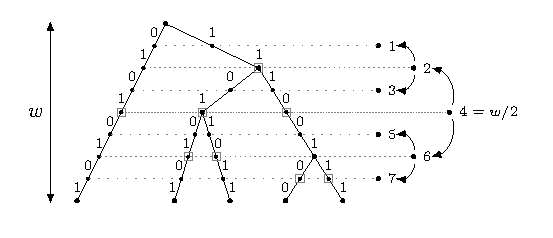
\includegraphics{binsearch_assoc_key_main}
\caption{The associated key $\alpha_e$ of an edge $e$:
we perform a binary search on the height of
$\lcp_S(q)$ in $T$. The \emph{associated key}
of an edge $e$ is the prefix of $\lcp_S(q)$ in which the
search first encounters the edge $e$. }
\label{fig:binsearch}
\end{figure}


The binary search needs $\log w$ steps, and 
since we assumed that $w$ is a power of two,
each step determines the next bit in the binary 
expansion of the \emph{length} of $\lcp_S(q)$.
Thus, the associated key of an edge $e$
can be computed in $O(1)$ time on a word RAM 
as follows: consider the $\log w$-bit binary 
expansions $\ell_u = |p_u|_2$ and  $\ell_v = |p_v|_2$ of the
\emph{lengths} of the prefixes
$p_u$ and $p_v$, and let $\ell'$ be the
longest common prefix of $\ell_u$ and
$\ell_v$. We need to determine the first
step when the binary search can distinguish between
$\ell_u$ and $\ell_v$. Since $\ell_u < \ell_v$,
and since the two binary expansions differ in the
first bit after $\ell'$,
it follows that $\ell_u$ begins with $\ell'0$ and
$\ell_v$ begins with $\ell'1$. Thus, let $\ell$ be obtained
by taking $\ell'$, followed by $1$ and
enough $0$'s to make a $\log w$-bit
word. Let $l$ be the number encoded by $\ell$.
Then, the associated key $\alpha_e$ consists of the 
first $l$ bits of $p_v$;
see~\cite{BelazzouguiBoVi10,Ehrhardt15,Ruzic09} for more details.

\paragraph{Hash Maps.}
Our data structure also makes extensive use of
hashing. In particular, we will maintain several
succinct hashtables that store additional
information for supporting fast queries.
For this, we will use a hashtable described
by Demaine~\etal~\cite{DemaineMePaPa06}.
The following theorem summarizes the properties
of their data structure.

\begin{theorem}
For any $r \geq 1$, there exists a dynamic dictionary that
stores entries with keys from $U$ and with associated
values of $r$ bits each.
The dictionary supports updates and queries in $O(1)$ time,
using $O(n \log\log (|U|/n) + nr)$ \emph{bits} of space.
The bounds for the space and the queries are
worst-case, the bounds for the updates hold with
high probability.\qed
\end{theorem}

\section{Static $\Delta$-fast Tries}
\label{sect:delta-fast_trie}

We are now ready to describe our data structure 
for the static case. In the next section, we will
discuss how to add support for insertions and
deletions.

\subsection{The Data Structure}
Our data structure is organized as follows:
let $S \subseteq U$, $|S| = n$, be given.
We store $S$ in a compressed trie
$T$. The leaves of $T$ are
linked in sorted order. Furthermore, 
for each node $v$ of $T$, let $T_v$ be the
subtree rooted at $v$. Then, $v$ stores pointers 
to the smallest and the largest leaf in 
$T_v$. To support the queries, we store 
three additional hash maps: $H_\Delta$, $H_z$,
and $H_b$.

First, we describe the hash map $H_\Delta$.
Set $m = \log\log w$. For
$i = 0, \dots, m$, we let
$h_i = 2^{2^i}$ and  
$d_i = w - h_i$. 
The hash map $H_\Delta$ stores the following
information: for each $s \in S$ and each
$d_i$, $i = 1, \dots, m$,
let $s_i = s_0 \dots s_{d_i-1}$ be the leftmost
$d_i$-bits of $s$ and let $e = (u,v)$ be
the edge of $T$ such that $s_i$ lies
on $e$.
Then, $H_\Delta$ stores the entry
$s_i \mapsto u$.

Next, we describe the hash map $H_z$.
It is defined similarly as the hash map
used for $z$-fast tries~\cite{BelazzouguiBoVi10,Ruzic09}.
For each edge $e$ of $T$, let $\alpha_e$ be
the associated key of $e$, as explained in 
Section~\ref{sec:prelim}.
Then, $H_z$ stores the entry $\alpha_e \mapsto e$.


Finally, the hash map $H_b$ is used to implement
a second layer of indirection that lets us achieve
linear space. It will be described below.

\subsection{The Predecessor Query}
\label{sec:staticquery}

Let $q \in U$ be the query, and let
$q^-$ and $q^+$ be the predecessor and
the successor of $q$ in $S$, as described above.
We first show how to get a running time
of $O(\log\log \Delta)$ for the queries, with  
$\Delta = |q - q^+|$.  In Theorem~\ref{thm:staticresult}, we will 
see that this can easily be improved
to $\Delta = \min\{|q - q^-|, |q - q^+|\}$.

The predecessor search works in several 
\emph{iterations}. In iteration $i$, we consider
the prefix $q_i$ that consists of the first $d_i$ 
bits of $q$.

First, we check whether 
$H_\Delta$ contains an entry for
$q_i$. If so, we know that $T$ contains
an edge $e$ such that $q_i$ lies on $e$.
Hence, $q_i$ must be  a prefix of $\lcp_S(q)$.
If one of the endpoints of $e$ happens to be
$\lca_T(q)$, we are done.
Otherwise, we consider the two edges emanating from  the lower
endpoint of $e$, finding the edge $e'$ that lies on
the path to $q$.
We take the associated key $\alpha_{e'}$ of $e'$,
and we use it to continue the binary search
for $\lca_T(q)$, as described in
Section~\ref{sec:prelim}. Since $|q_i| = d_i$,
this binary search takes 
$O(\log (w - d_i)) = O(\log h_i)$ steps to complete.
Once the lowest common ancestor $v = \lca_T(q)$ is 
at hand,  we can find the predecessor of $q$ in $O(1)$ 
additional time: it is either the rightmost element in $T_v$,
the predecessor of the leftmost element in $T_v$, or the 
rightmost element in the left subtree of $v$. Given the 
pointers stored with $v$ and the leaves of $T$, all these
nodes can be found in $O(1)$ time.

If $H_\Delta$ contains no entry for
$q_i$ and if $q_i$ does not consist
of all $1$'s, we check if $H_\Delta$ contains
an entry for $q_i + 1$.
Notice that $q_i+1$ is the successor of $q_i$. 
If such an entry exists,
we first obtain $u = H_\Delta[q_i +1]$, and the child $v$ of 
$u$ such that $q_i + 1$ lies on the edge $e = (u,v)$.
Then, we follow the pointer to the leftmost element of
$T_v$. This is the successor $q^+$ of $q$. 
The predecessor $q^-$ can then be found by following the 
leaf pointers. This takes $O(1)$ time overall.

Finally, if there is neither an entry for $q_i$
nor for $q_i+1$, we continue 
with iteration $i+1$, see Figure~\ref{fig:query}.

\begin{figure}
\centering
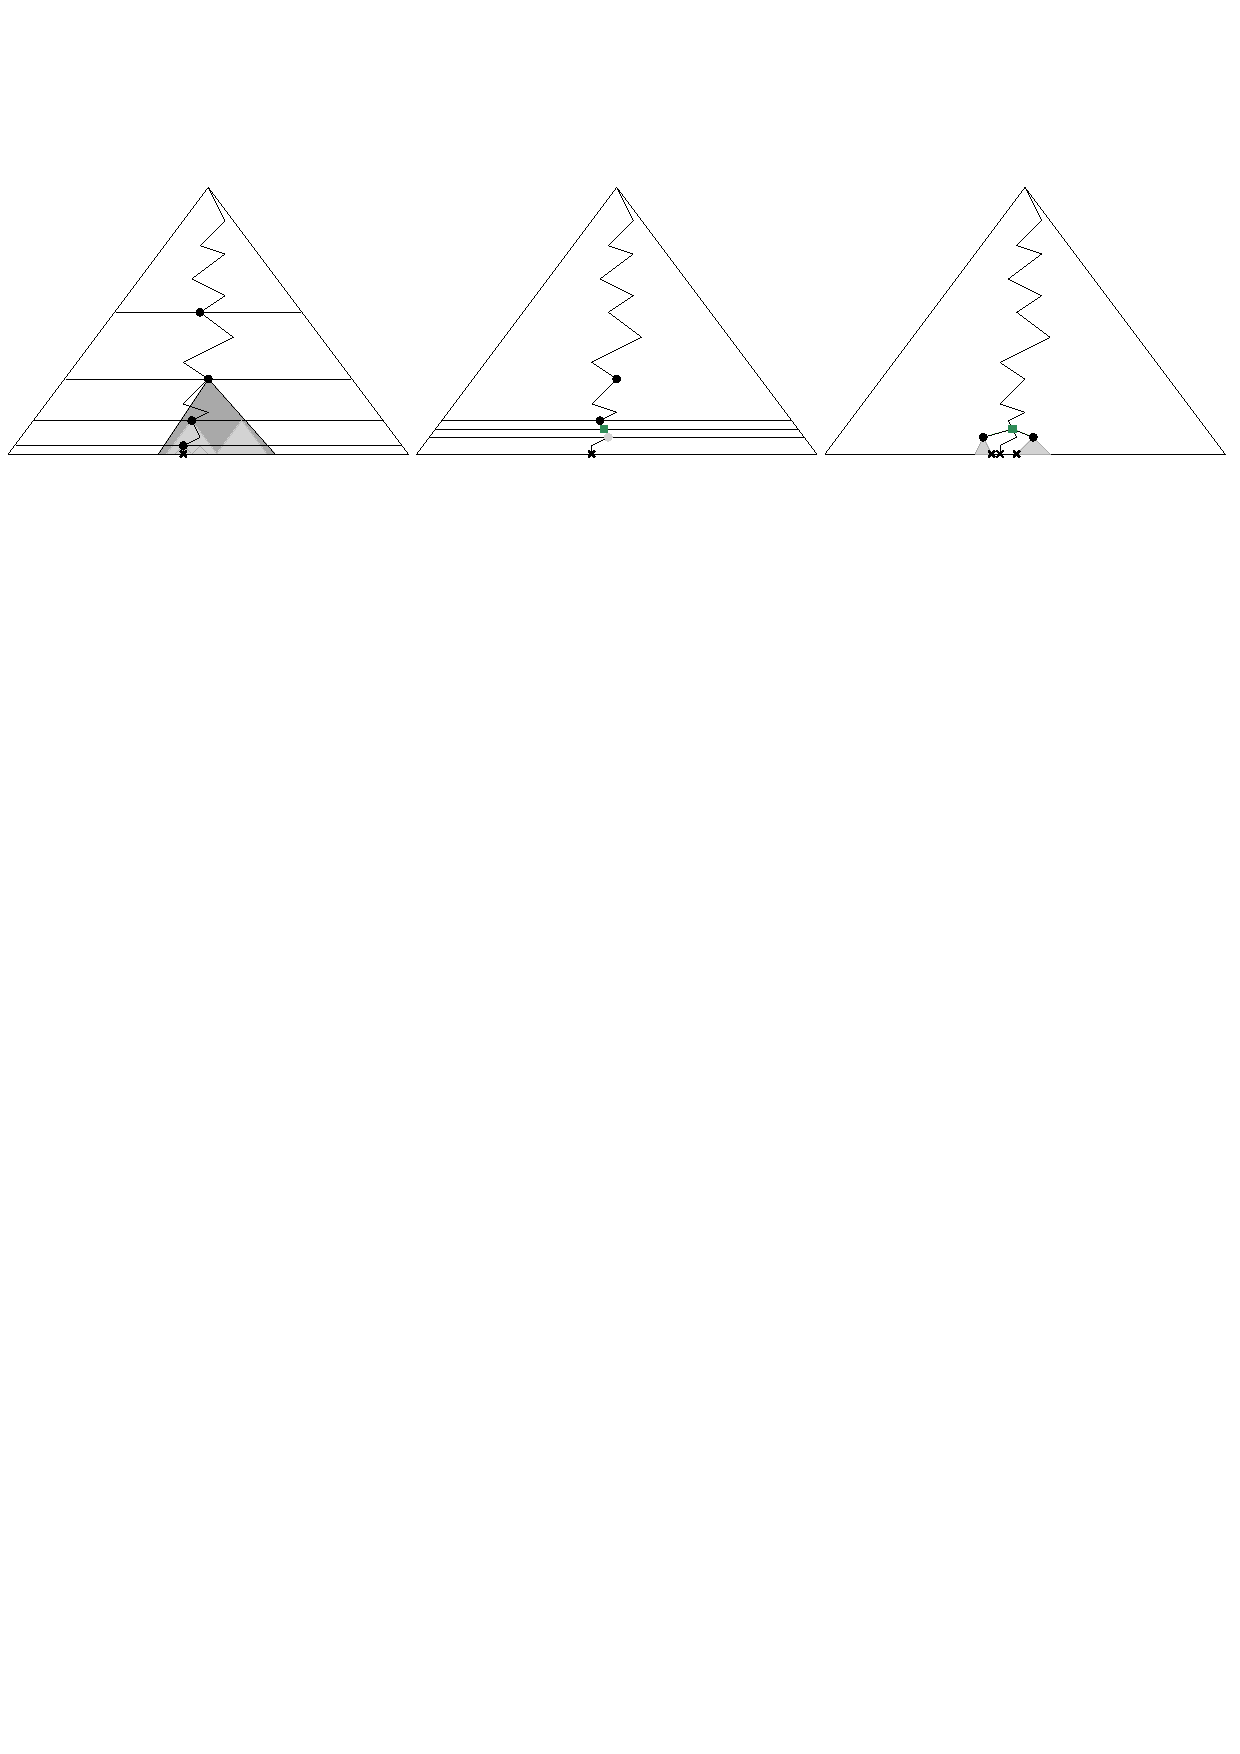
\includegraphics[scale=0.5]{query}
\caption{The query algorithm: first we perform an
exponential search from the lowest level, to find a prefix
of $q_k$  or $q_k+1$ (left). If a prefix $q_{k}$ is found,
we perform a binary search for $\lca_T(q)$ (middle), which can then
be used to find the predecessor and successor of $q$ (right). If
a prefix $q_k+1$ is found, the successor and predecessor 
can be found immediately (not shown).}
\label{fig:query}
\end{figure}

From the above discussion, it follows that
the total time for the predecessor
query is $O(k + \log h_k)$, where $k$ is the number of 
iterations and $\log h_k$ is the worst-case time 
for the predecessor search once one of the lookups 
in an iteration succeeds. 
By our predecessor algorithm, we know that $S$ contains no element with
prefix $q_{k-1}$ or $q_{k-1} + 1$, but an element with
prefix $q_k$ or $q_k + 1$. Thus, there must be
at least $2^{w - d_k} = 2^{h_k}$ consecutive elements in 
$U\setminus S$ following $q$. By our definition of $h_k$, it follows that
$\Delta \geq 2^{h_{k-1}} = 2^{2^{2^{k-1}}}$, so 
$k \leq 1 + \log\log\log \Delta$.
Furthermore, since $h_k = 2^{2^k} = \left(2^{2^{k-1}}\right)^2 
=  (h_{k-1})^2$, 
it follows that $h_k = O(\log^{2} \Delta)$.

\subsection{Obtaining Linear Space}
We now analyze the space requirement for our
data structure.
Clearly,  the  trie $T$ and the
hash map $H_z$ require $O(n)$ words of space.
Furthermore, as described so far, the number of 
words needed for
$H_\Delta$ is $O(n \log\log w)$, since 
we store at most $n$ entries for each 
height $h_i$, $i = 0, \dots, m = \log\log w$.

Using a trick due to P\v{a}tra\c{s}cu~\cite{Patrascu10}, 
we can introduce another level of indirection to reduce 
the space requirement to  $O(n)$.
The idea is to store in $H_\Delta$ the \emph{depth}
$d_u$ of each branch node $u$ in $T_\Delta$, instead of storing 
$u$ itself (here, we mean the depth in the
original trie, i.e., the length of the prefix $p_u$). 
We then use an additional hash map 
$H_b$ to obtain $u$.
This is done as follows:
when trying to find the branch node $u$ for a given
prefix $q_i$, we 
first get the depth $d_u = |p_u|$ of $u$ 
from $H_\Delta$. After that, we look up the branch
node $u = H_b[q_0 \dots q_{d_u-1}]$ from the hash map 
$H_b$. Finally, we check whether $u$ is actually the 
lowest branch node of $q_i$. If any of those steps fails,
we return $\bot$.

Let us analyze the needed space: clearly, $H_b$ needs
$O(n)$ words, since it stores $O(n)$ entries.
Furthermore,
we have to store $O(n \log\log w)$ entries in 
$H_\Delta$, each mapping a prefix $q_i$ to the depth of 
its lowest branch node. This depth requires
$\lceil \log w \rceil$ bits.
By Theorem~\ref{thm:succinct_retrieval_only_hashtable},
a retrieval only hash map for $n'$ items and $r$ bits 
of data needs $O(n'\log\log \frac{|U|}{n'} + n'r)$ bits.
Therefore, the space 
\emph{in bits} for $H_\Delta$ is proportional to
\begin{align*}
&\phantom{=} n \log\log w \cdot \log\log \frac{|U|}{n \log\log w} +
n \log\log w \cdot \lceil \log w \rceil\\
&= O(n \log\log w \cdot \log w)\\
&= o(n\cdot w),
\end{align*}
using $n' = n\log\log w$, $r = \lceil \log w \rceil$ and $w = \log |U|$. 
Thus, we can store $H_\Delta$ in 
$O(n)$ words of $w$ bits each. The following lemma summarizes
the discussion

\begin{lemma}
\label{lemma:delta_linear_space}
The $\Delta$-fast trie needs $O(n)$ words space.
\end{lemma}

\subsection{Putting it Together}

We can now obtain our result for the static predecessor problem.

\begin{theorem}\label{thm:staticresult}
Let $U = \{0, \dots, 2^{w}-1\}$ and let
$S \subseteq U$, $|S| = n$.
The static $\Delta$-fast trie for $S$ requires
$O(n)$ words of space, and it can answer
a static predecessor query for an element $q \in U$ on $S$ in time
$O(\log \log \min\{|q-q^-|, |q-q^+|\})$,
where $q^-$ and $q^+$ denote the predecessor
and successor of $q$ in $S$.
The preprocessing time is 
$O(n \log\log \log |U|)$, assuming that
$S$ is sorted.
\end{theorem}

\begin{proof}
The regular search for $q \in S$ can be done in 
$O(1)$ time by a lookup in $H_z$. 
We have seen that the predecessor of $q$
can be found in $O(\log \log |q-q^+|)$ time.
A symmetric result also holds for 
successor queries.
In particular, we can achieve query time 
$O(\log \log |q-q^-|)$  by checking for
$H_\Delta[q_i-1]$ instead of $H_\Delta[q_i+1]$ in the 
query algorithm. 

By interleaving the two searches,
we obtain the desired running time of 
$O(\log\log \min\{|q - q^-|, |q - q^+|\})$. 
Of course, in a practical implementation, it would be 
more efficient to check directly for $H_\Delta[q_i-1]$
and $H_\Delta[q_i+1]$ in the query algorithm.

The trie $T$ and the hash maps $H_z$
and $H_b$ can be computed in $O(n)$ time, given that
$S$ is sorted.
Thus, the preprocessing time is dominated by the time to fill the 
hash map $H_\Delta$.  Hence, the preprocessing needs
$O(n\log\log\log |U|)$ steps, because $O(n\log\log w)$ nodes 
have to be
inserted into $H_\Delta$. 
By Lemma~\ref{lemma:delta_linear_space}, the space requirement
is linear.
\end{proof}

\section{Dynamic $\Delta$-fast tries}

We will now explain how to extend our data
structure to the dynamic case. 
The basic data structure remains the same, but
we need to update the hashtables and the trie $T$
after each insertion and deletion.
In particular, our data structure requires that
for each $v$ in $T_v$, we can access the 
leftmost and the rightmost node
in the subtree $T_v$.
In the static case, this could be done simply
by maintaining explicit pointers from each node
$v \in T$ to these nodes in $T_v$, letting us find
the nodes in $O(1)$ time.
In the dynamic case, we will maintain a data structure
which allows finding and updating these nodes in
in $O(\log\log \Delta)$ time.

\subsection{Computing Lowest Common Ancestor}

To perform the update operation, we need a
procedure to compute the lowest common ancestor 
$\lca_T(q)$ for any given element $q \in U$. 
For this, we proceed as in the query algorithm from 
Section~\ref{sec:staticquery}, but skipping 
the lookups for $H_\Delta[q_i-1]$ and
$H_\Delta[q_i+1]$. By the analysis in 
Section~\ref{sec:staticquery}, this will find 
$\lca_T(q)$ in time $O(\log \log l)$, where $l$
is height of $\lca_T(q)$ in $T$.

Unfortunately, it may happen that this height $l$ is as large as $w$,
even if $q$ is close to an element in the current set $S$.
To get around this, we use a trick of Bose~\etal~\cite{BoseDoDuHoMo13}.
Namely, their idea is to perform a random shift of the universe. 
More precisely, we pick a random number $r \in U$, and we
add $r$ to all query and update elements that appear in 
the data structure (modulo $|U|$).

\begin{lemma}[Lemma 4 in \cite{BoseDoDuHoMo13}]
\label{lemma:delta_lca_loglog_delta}
Let $x, y \in U$ be two fixed elements in $U$.
Let $r \in U$ be picked uniformly at random.
After a random shift of $U$ by $r$, the 
expected height of the lowest common ancestor of 
$x$ and $y$ in a compressed trie is $O(\log|x-y|)$.\qed
\end{lemma}

\begin{corollary}
\label{cor:delta_fast_expected_lca}
Let $S \subseteq U$ and let $T$ be a randomly
shifted $\Delta$-fast trie storing $S$.
Let $q \in U$. 
We can find $\lca_T(q)$ in expected time $O(\log\log \Delta)$,
where $\Delta = \min\{|q - q^+|, |q-q^-|\}$, the elements 
$q^+$ and $q^-$ being the predecessor and successor of $q$ in $S$.
The expectation is
over the random choice of the shift $r$. 
\end{corollary}

\begin{proof}
Suppose without loss of generality that $\Delta = |q - q^+|$.
By Lemma~\ref{lemma:delta_lca_loglog_delta},
the expected height $h_k$ of the lowest common ancestor of $q$ and $q^+$
is $O(\log \Delta)$.
We perform the doubly exponential
search on the prefixes of $q$, as in Section~\ref{sec:staticquery} 
(without checking $q_i+1$) to find the height $h_k$. After
that, we  resume the search for $\lca_T(q)$ on the 
remaining $h_k$ bits. Since $h_k = O(\log \Delta)$ in expectation,
it follows by Jensen's inequality that the number $k$
of loop iterations to find  $h_k$ is $O(\log\log\log \Delta)$
in expectation. Thus, the expected running time is proportional to
$k + \log h_k = O(\log\log\Delta)$. 
\end{proof}

\subsection{Managing the Left- and Rightmost Elements 
of the Subtrees}

We also need to maintain for each node $v \in T$ the
leftmost and the rightmost element in the subtree $T_v$.
In the static case, it suffices to have direct pointers
from $v$ to the respective leaves, but
in the dynamic case, we need an additional data structure. 

\begin{figure}
\centering
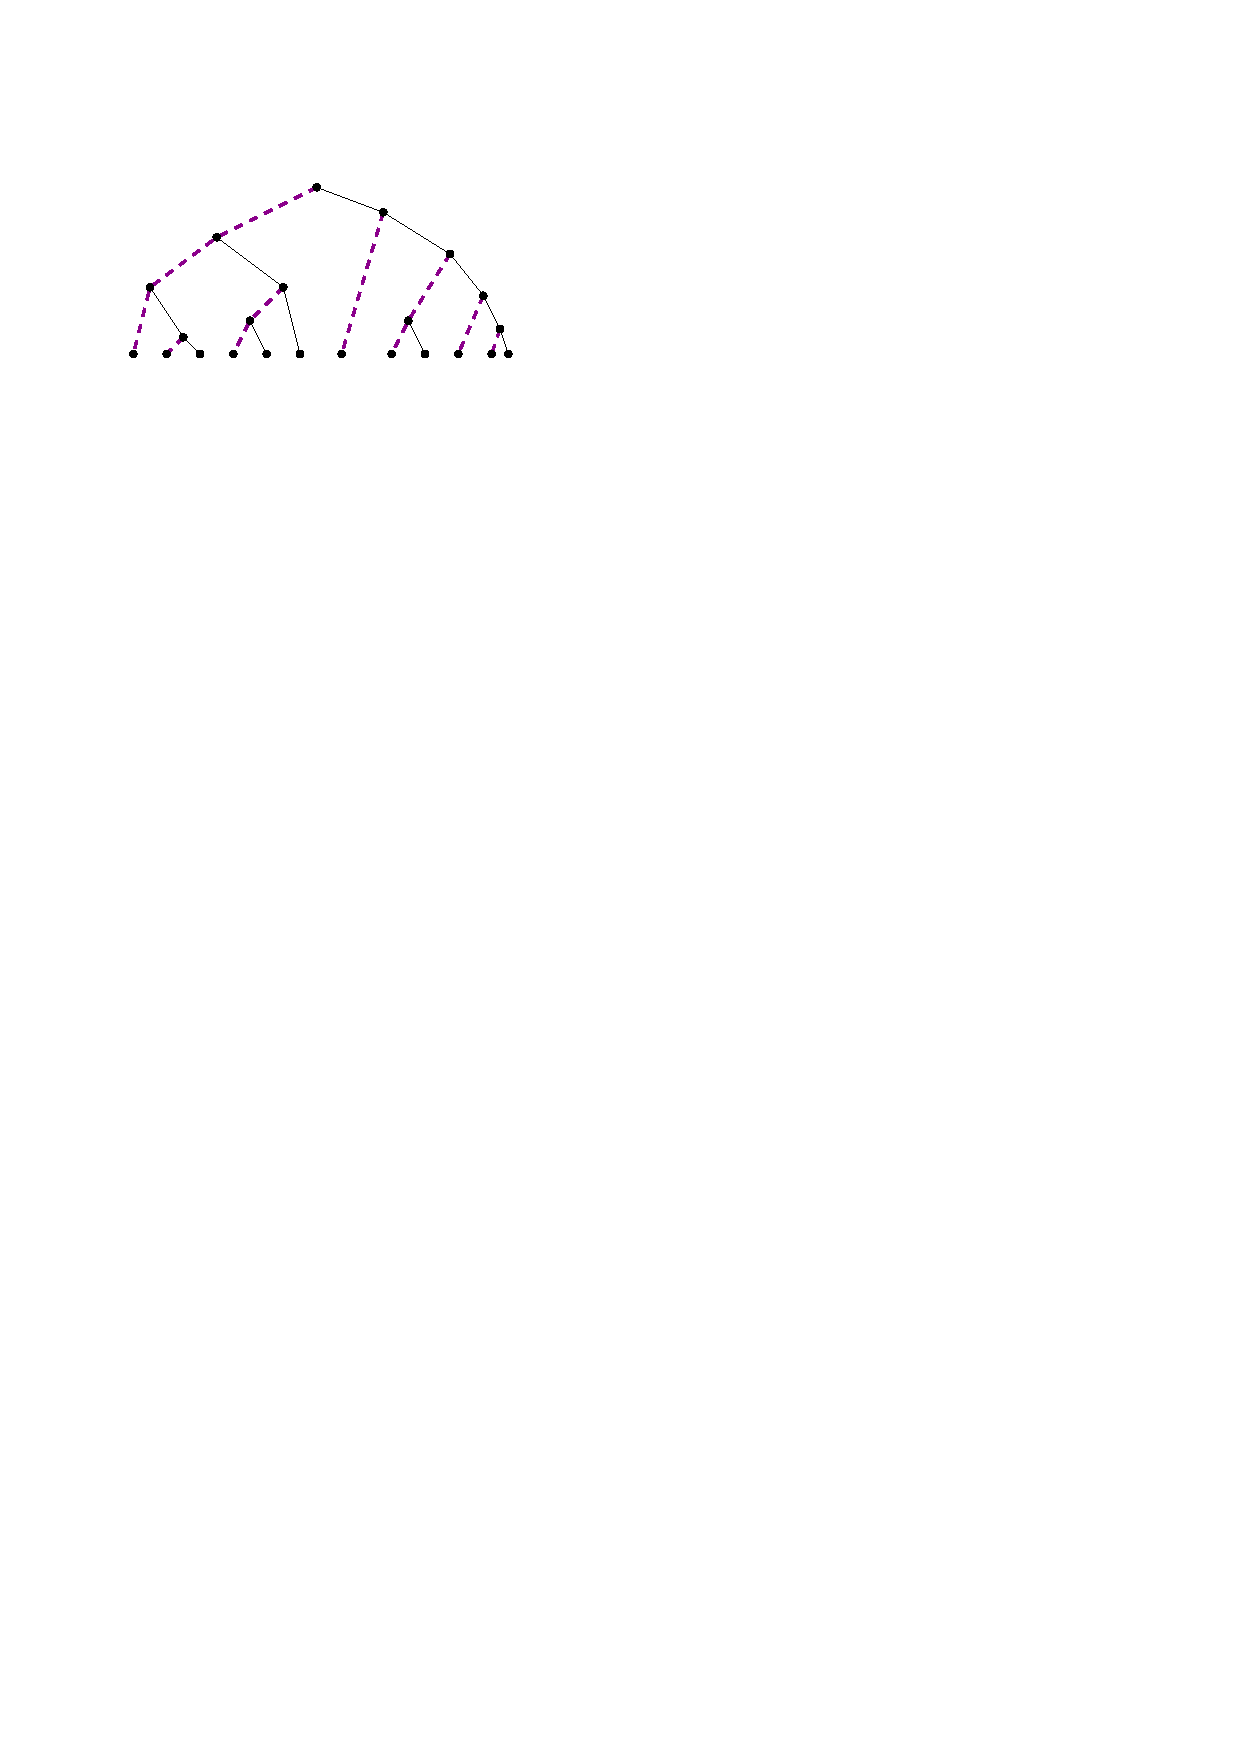
\includegraphics{pathdecomp}
\caption{For each leaf $v'$ of $T$, the nodes
$v \in T$ for which $v$ is the leftmost leaf in $T_v$
if a subpath of a root-to-leaf path in $T$. Considering these
subpaths for all leaves in $T$, we obtain a \emph{path decomposition}
of $T$ (shown in bold).}
\label{fig:pathdecomp}
\end{figure}
To do this, we observe the following: let $v' \in T$ be 
a leaf in $T$. Then, $v'$ is the leftmost (or rightmost)
leaf in the subtrees of at most $w$ ancestors $v$ of $v'$.
Furthermore, all these nodes form a subpath (more precisely,
a prefix) of the path from $v$ to the root, see Figure~\ref{fig:pathdecomp}.
Hence, if we maintain the nodes of 
this subpath in a concatenable queue data structure
(realized by, e.g., a balanced binary tree)~\cite{PreparateSh85},
we can obtain $O(\log w)$ update and query time
to find the leftmost (or rightmost) element in $T_v$
for each $v \in T$.
However, we need that the update and query time for this
data structure
depend on the height $h_i$ (i.e, the remaining bits) 
of the query node $v$.
Thus, we partition the possible heights
$\{0, 1, \dots, w\}$ of the nodes on a 
subpath into the sets
$T_{-1} = \{0\}$, $T_i =[2^i, 2^{i+1})$, for $i = 0,\dots,\log w-1$, 
and $T_{\log w} = \{w\}$.
Each set is managed by a balanced binary tree, and the 
roots of the trees are linked together. The height of the $i$-th binary 
search tree is $\log |T_i| = O(i)$. Furthermore, if a query node
of height $h$ is given, 
the set $T_{\lfloor \log h \rfloor}$ is responsible for it, see 
Figure~\ref{fig:queryds}.
\begin{figure}
\centering
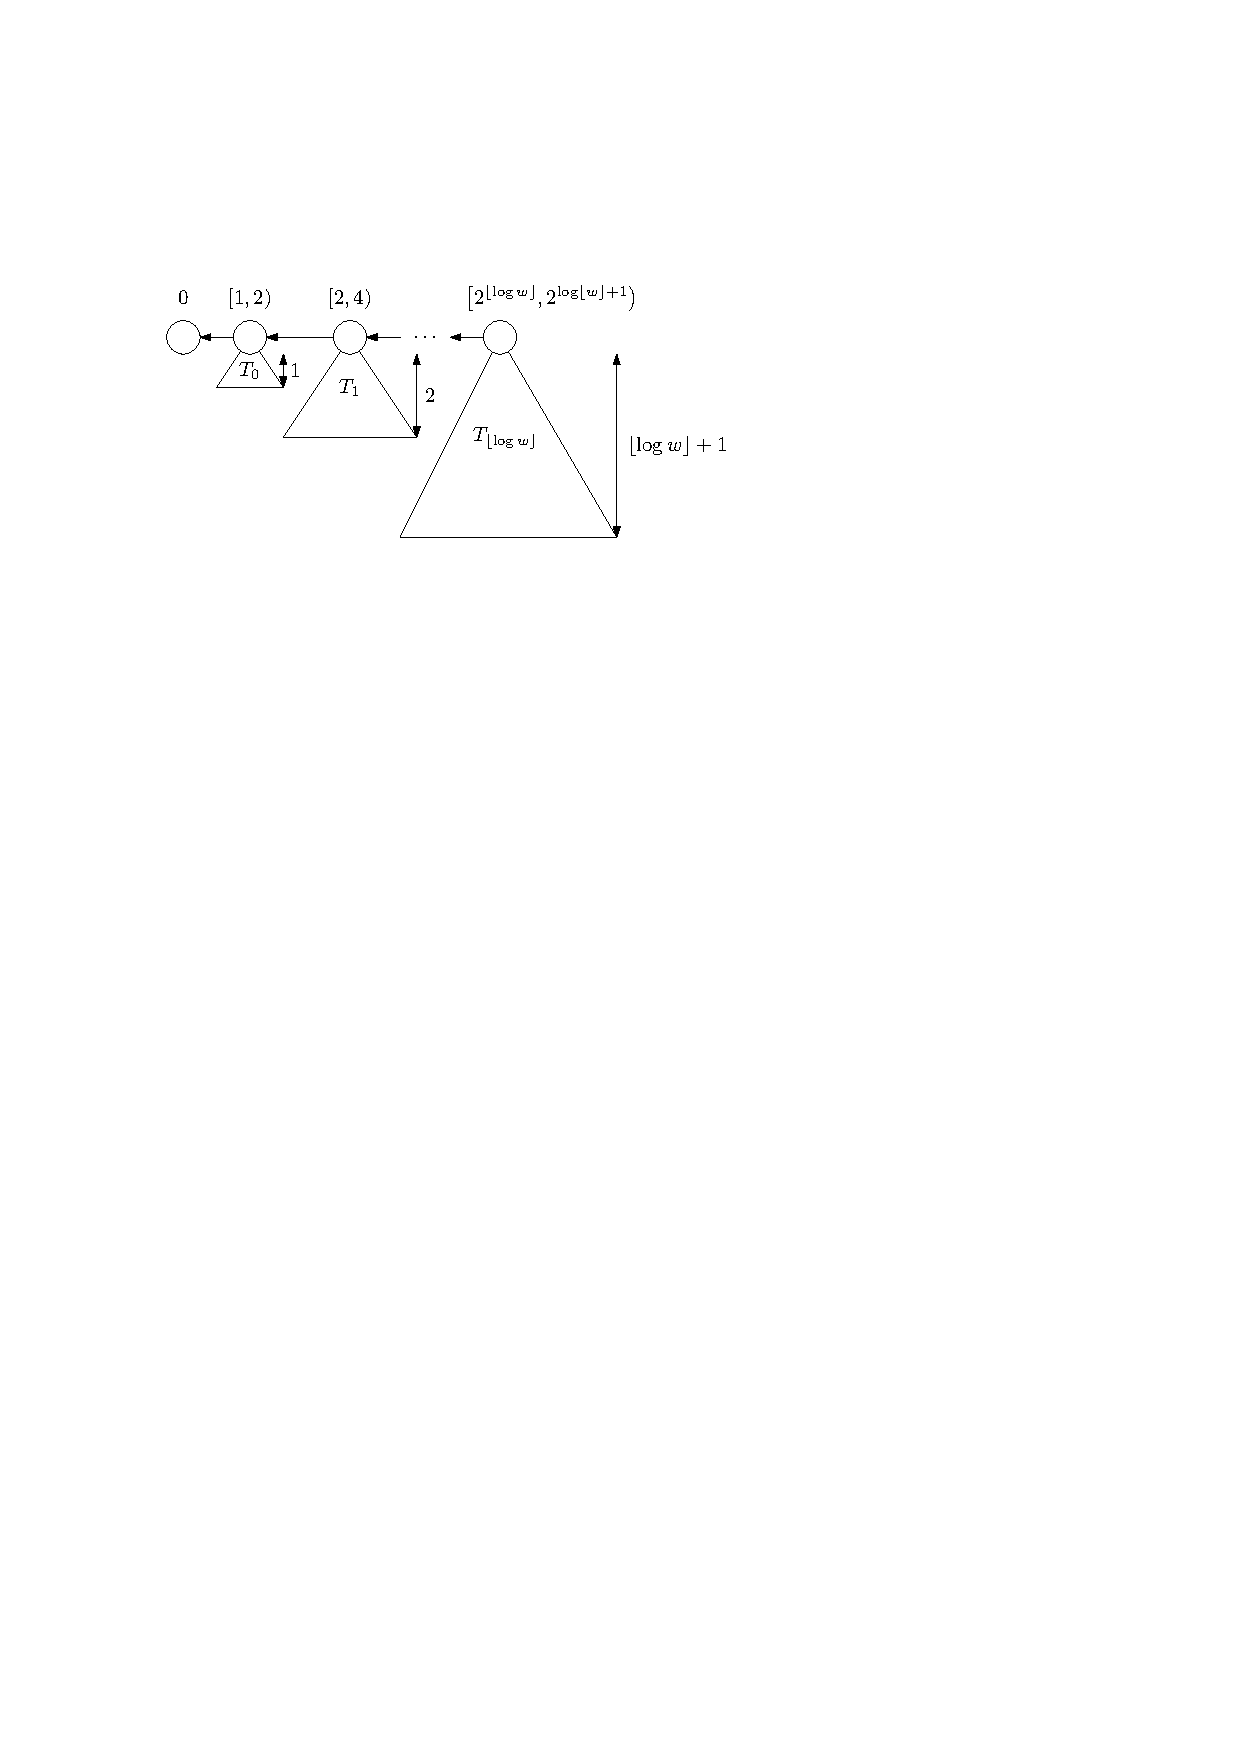
\includegraphics{queryds}
\caption{The data structure for a subpath. We group the nodes
in the subpath according to their heights, where the groups
grow exponentially in size. Each group is represented by a
balanced tree. The roots are joined in a linked
list. With this data structure, a node $v$ of height $h$ can
find the leftmost leaf in the subtree $T_v$ in time $O(\log h)$.}
\label{fig:queryds}
\end{figure}


Moreover, $T_{-1}$ is a leaf (the depth of that node is $w$) 
in the trie and therefore the minimum of the whole subpath. Thus, 
the minimum of a subpath can be found from a given node 
$v \in T_i$ in $O(i)$ time by following the
pointers to the root of $T_i$ and the pointers down to $T_{-1}$.

If a node $v$ has $h_k = O(\log \Delta)$ height (remaining bits), 
the node is within
the tree $T_{\lfloor \log h_k \rfloor}$. Thus, it takes 
$O(\log h_k) = O(\log\log\Delta)$ time to find the leftmost
or rightmost leaf in $T_v$.

Furthermore, we can support the following update operations:
(i) \textbf{split}: given a subpath $\pi$ and a node $v$ on $\pi$, split 
the representation of $\pi$ into two representations, one for the 
\emph{lower} subpath from the leaf up to the child of $v$, and
one for the \emph{upper} subpath starting from $v$; and (ii) 
\textbf{join}: given a
representation of an upper subpath starting at a node $v$ obtained 
from an operation of type (i), and a representation for 
a lower subpath up to a child of $v$, join the two representations
into the representation for a joint subpath.
Given the data structure, we can support
both \textbf{split} and \textbf{join} in
 $O(\log h)$ time, where $h$ is the height of 
the node $v$ where the operation occurs. 
This decomposition of $T$ into dynamically changing suppaths
is similar to the \emph{preferred paths decomposition} of
Tango trees~\cite{DemaineHaIaPa07}.

\subsection{Performing an Update}

We know from the Lemma~\ref{lemma:delta_lca_loglog_delta}, that 
the lowest common ancestor of a query element $q$ has expected 
height $h_k = O(\log \Delta)$.

\begin{lemma}
\label{lemma:delta_insert}
Let $S \subseteq U$, and let $T$ be
a randomly shifted $\Delta$-fast tree for 
$S$.  Let $q \in U$ be fixed.
We can insert or delete $q$ into $T$
in $O(\log \log \Delta)$ expected time, where the expectation is 
over the random choice of the shift $r$.
\end{lemma}

\begin{proof}
To insert $q$ into $T$, we need to split an edge $(u,v)$ of $T$ into
two edges $(u,b)$ and $(b,v)$. This creates
exactly two new nodes in $T$, an inner node and a leaf node. 
The branch node is exactly $\lca_T(q)$, and it has expected height 
$h_k = O(\log \Delta)$, by Lemma~\ref{lemma:delta_lca_loglog_delta}. 
Thus, it will
take $O(\log\log \Delta)$ expected time to find
the edge $(u,v)$, by
Corollary~\ref{cor:delta_fast_expected_lca}.

Once the edge $(u,v)$ is found, the hash maps $H_z$ and $H_u$ 
can then be updated in constant time.
Now let us consider the update time of the 
hash map $H_\Delta$. Recall that
$H_\Delta$ stores the lowest branch nodes for all prefixes
of the elements in $S$ that have certain lengths.
This means that all prefixes on the edge $(b,v)$ which 
are stored in the hash map $T_\Delta$ need to
be updated. Furthermore, prefixes at certain depths which 
are on the new edge $(b,q)$ need to
be added. For the edge $(b,v)$, we will enumerate 
all prefixes at certain depths, but we will select only those that 
lie on the edge $(b,v)$. This needs
$O(\log\log\log\Delta)$ insertions and updates in total: we
have to insert the prefixes $q_0 \dots q_{d_i}$ for all 
$i \geq 1$ with $d_i < |b|$. Since we defined 
$d_i = w - h_i = w - 2^{2^i}$, 
and since $|b| = w - O(\log \Delta)$, 
we have that $d_i \leq |b|$ as soon as 
$c \log\Delta < 2^{2^i}$. This holds for 
$i > \log\log (c\log \Delta)$, and hence $i =
\Theta(\log\log\log\Delta)$.

After that, the leftmost and rightmost elements for the subtrees
of $T$ have to be updated. For this, we need to add one
subpath for the new leaf $q$, and we may need to split
a subpath at a node of height $h_k = O(\log \Delta)$ and join
the resulting upper path with the newly created subpath. As we
have seen, this takes $O(\log h_k) = O(\log \log \Delta)$ time.

The operations for deleting an element $q$ from $S$ are symmetric.
\end{proof}

The following theorem summarizes our result.

\begin{theorem}
Let $r \in U$ be picked uniformly at random.
After performing a shift of $U$ by $r$, 
the $\Delta$-fast trie provides a data structure for the
dynamic predecessor problem such that the 
query operations take $O(\log \log \Delta)$ worst-case time and 
the update operations need $O(\log \log \Delta)$ expected
time, for $\Delta = \min \{|q-q^+|, |q-q^-|\}$, where $q$ is the
requested element and $q^+$ and $q^-$ are the predecessor and
successor of $q$ in the current set $S$. At any point in time, 
the data structure needs $O(n)$ words of space, where $n = |S|$.
\end{theorem}

\section{Applications}

Bose~\etal~\cite{BoseDoDuHoMo13} describe how to combine their structure
with a technique of Chan~\cite{Chan02} and random 
shifting~\cite[Chapter~11]{HarPeled11} for obtaining a data structure for 
distance-sensitive
approximate nearest neighbor queries on a grid.
More precisely, let $d \in \N$ be the fixed dimension, 
$U = \{0, \dots, 2^{w}-1\}$ be the universe, and
let $\eps > 0$ be given.
The goal is to maintain a dynamic set $S \subseteq U^d$ under
insertions, deletions, and \emph{$\eps$-approximate
nearest neighbor queries}: given a query point $q \in U^d$,
find a $p \in S$ with $d_2(p,q) \leq (1+\eps)d_2(p, S)$.
Plugging our $\Delta$-fast tries into the structure of
Bose~\etal~\cite[Theorem~9]{BoseDoDuHoMo13}, we can
immediately improve the space requirement of their structure to linear:
\begin{theorem}
Let $U = \{0, \dots, 2^w-1\}$ and let $d$ be a constant.
Furthermore, let $\eps > 0$ be given.
There exists a data structure that supports $(1+\eps)$-approximate
nearest neighbor queries over a subset $S \subseteq U^d$ in 
$(1/\eps^d)\log\log \Delta)$ expected time and insertions and deletions
of elements of $U^d$ in $O(\log\log \Delta)$ expected time.
Here, $\Delta$ denotes the Euclidean distance between the query element
and $S$. At any point in time, the data structure requires $O(n)$
words of space, where $n  = |S|$.
\end{theorem}

As a second application, Bose~\etal~\cite{BoseDoDuHoMo13}
present a data structure for dominance queries on a grid,
based on a technique of Overmars~\cite{Overmars88}.
Again, let $U = \{0, \dots, 2^w-1\}$, and let $S \subseteq U^2$,
$|S| = n$ be given. The goal is to construct a data structure
for \emph{dominance queries} in $S$. That is, given a query point
$q \in U^2$, find all points $p$ in $S$ that \emph{dominate} $q$,
i.e., for which we have $p_x \geq q_x$ and $p_y \geq q_y$, there
$p_x$, $p_y$ and $q_x$, $q_y$ are the $x$- and $y$-coordinates 
of $p$ and $q$.

Again, using $\Delta$-fast tries, we can immediately improve the
space requirement for the result of 
Bose~\etal~\cite[Theorem~10, Corollary~13]{BoseDoDuHoMo13}.

\begin{theorem}
Let $U = \{0, \dots, 2^w-1\}$, and let $S \subseteq U^2$, $|S|=n$
be given. There exists a data structure that reports the points in $S$
that dominate a given query point $q = (a,b) \in U^2$ in expected time
$O(\log\log(h+v) + k)$, where $h = 2^w - a$, $v = 2^2-b$, and $k$
is the number of points in $S$ dominated by $q$.
The data structure uses $O(n \log n)$ space.
\end{theorem}
\section{Conclusion}

We present a new data structure for local searches
in bounded universes. This structure now interpolates
seamlessly between hashtables and van-Emde-Boas trees,
while requiring only a linear number of words. This provides
an improved, and in our opinion also slightly simpler, version
of a data structure by Bose \etal~\cite{BoseDoDuHoMo13}.
All the operations of our structure can be
presented explicitly in pseudocode. This can be found in the
Master's thesis of the first author~\cite{Ehrhardt15}.

\bigskip
\noindent\textbf{Acknowledgments.}
We thank the anonymous reviewers for numerous
insightful comments that improved the quality of the paper.
\wolfgang{TODO}

\hyphenation{ Vi-gna Sa-ba-di-ni Kath-ryn Ker-n-i-ghan Krom-mes Lar-ra-bee
  Pat-rick Port-able Post-Script Pren-tice Rich-ard Richt-er Ro-bert Sha-mos
  Spring-er The-o-dore Uz-ga-lis }


\bibliographystyle{abbrv}
\bibliography{journal}

\end{document}
